\documentclass[]{article}

\usepackage{graphicx,type1cm,eso-pic,color}
\usepackage[spanish]{babel} %%%% for


\makeatletter
          \AddToShipoutPicture{
            \setlength{\@tempdimb}{.95\paperwidth}
            \setlength{\@tempdimc}{.5\paperheight}
            \setlength{\unitlength}{1pt}
            \put(\strip@pt\@tempdimb,\strip@pt\@tempdimc){
        \makebox(0,0){\rotatebox{-90}{\textcolor[gray]{0.90}
        {\fontsize{.65cm}{.5cm}\selectfont{\rm Dae-Jin Lee}}}}
            }
        }
          \AddToShipoutPicture{
            \setlength{\@tempdimb}{.50\paperwidth}
            \setlength{\@tempdimc}{.95\paperheight}
            \setlength{\unitlength}{1pt}
            \put(\strip@pt\@tempdimb,\strip@pt\@tempdimc){
        \makebox(0,0){\rotatebox{0}{\textcolor[gray]{0.90}
        {\fontsize{.5cm}{.5cm}\selectfont{\rm Curso de Estad\'istica b\'asica para Data Scientist  - @datahack}}}}
            }
        }
\makeatother

\def\tightlist{}

\usepackage{lmodern}
\usepackage{amssymb,amsmath}
\usepackage{ifxetex,ifluatex}
\usepackage{fixltx2e} % provides \textsubscript
\ifnum 0\ifxetex 1\fi\ifluatex 1\fi=0 % if pdftex
  \usepackage[T1]{fontenc}
  \usepackage[utf8]{inputenc}
\else % if luatex or xelatex
  \ifxetex
    \usepackage{mathspec}
    \usepackage{xltxtra,xunicode}
  \else
    \usepackage{fontspec}
  \fi
  \defaultfontfeatures{Mapping=tex-text,Scale=MatchLowercase}
  \newcommand{\euro}{???}
\fi
% use upquote if available, for straight quotes in verbatim environments
\IfFileExists{upquote.sty}{\usepackage{upquote}}{}
% use microtype if available
\IfFileExists{microtype.sty}{%
\usepackage{microtype}
\UseMicrotypeSet[protrusion]{basicmath} % disable protrusion for tt fonts
}{}
\usepackage{color}
\usepackage{fancyvrb}
\newcommand{\VerbBar}{|}
\newcommand{\VERB}{\Verb[commandchars=\\\{\}]}
\DefineVerbatimEnvironment{Highlighting}{Verbatim}{commandchars=\\\{\}}
% Add ',fontsize=\small' for more characters per line
\usepackage{framed}
\definecolor{shadecolor}{RGB}{248,248,248}
\newenvironment{Shaded}{\begin{snugshade}}{\end{snugshade}}
\newcommand{\KeywordTok}[1]{\textcolor[rgb]{0.13,0.29,0.53}{\textbf{{#1}}}}
\newcommand{\DataTypeTok}[1]{\textcolor[rgb]{0.13,0.29,0.53}{{#1}}}
\newcommand{\DecValTok}[1]{\textcolor[rgb]{0.00,0.00,0.81}{{#1}}}
\newcommand{\BaseNTok}[1]{\textcolor[rgb]{0.00,0.00,0.81}{{#1}}}
\newcommand{\FloatTok}[1]{\textcolor[rgb]{0.00,0.00,0.81}{{#1}}}
\newcommand{\ConstantTok}[1]{\textcolor[rgb]{0.00,0.00,0.00}{{#1}}}
\newcommand{\CharTok}[1]{\textcolor[rgb]{0.31,0.60,0.02}{{#1}}}
\newcommand{\SpecialCharTok}[1]{\textcolor[rgb]{0.00,0.00,0.00}{{#1}}}
\newcommand{\StringTok}[1]{\textcolor[rgb]{0.31,0.60,0.02}{{#1}}}
\newcommand{\VerbatimStringTok}[1]{\textcolor[rgb]{0.31,0.60,0.02}{{#1}}}
\newcommand{\SpecialStringTok}[1]{\textcolor[rgb]{0.31,0.60,0.02}{{#1}}}
\newcommand{\ImportTok}[1]{{#1}}
\newcommand{\CommentTok}[1]{\textcolor[rgb]{0.56,0.35,0.01}{\textit{{#1}}}}
\newcommand{\DocumentationTok}[1]{\textcolor[rgb]{0.56,0.35,0.01}{\textbf{\textit{{#1}}}}}
\newcommand{\AnnotationTok}[1]{\textcolor[rgb]{0.56,0.35,0.01}{\textbf{\textit{{#1}}}}}
\newcommand{\CommentVarTok}[1]{\textcolor[rgb]{0.56,0.35,0.01}{\textbf{\textit{{#1}}}}}
\newcommand{\OtherTok}[1]{\textcolor[rgb]{0.56,0.35,0.01}{{#1}}}
\newcommand{\FunctionTok}[1]{\textcolor[rgb]{0.00,0.00,0.00}{{#1}}}
\newcommand{\VariableTok}[1]{\textcolor[rgb]{0.00,0.00,0.00}{{#1}}}
\newcommand{\ControlFlowTok}[1]{\textcolor[rgb]{0.13,0.29,0.53}{\textbf{{#1}}}}
\newcommand{\OperatorTok}[1]{\textcolor[rgb]{0.81,0.36,0.00}{\textbf{{#1}}}}
\newcommand{\BuiltInTok}[1]{{#1}}
\newcommand{\ExtensionTok}[1]{{#1}}
\newcommand{\PreprocessorTok}[1]{\textcolor[rgb]{0.56,0.35,0.01}{\textit{{#1}}}}
\newcommand{\AttributeTok}[1]{\textcolor[rgb]{0.77,0.63,0.00}{{#1}}}
\newcommand{\RegionMarkerTok}[1]{{#1}}
\newcommand{\InformationTok}[1]{\textcolor[rgb]{0.56,0.35,0.01}{\textbf{\textit{{#1}}}}}
\newcommand{\WarningTok}[1]{\textcolor[rgb]{0.56,0.35,0.01}{\textbf{\textit{{#1}}}}}
\newcommand{\AlertTok}[1]{\textcolor[rgb]{0.94,0.16,0.16}{{#1}}}
\newcommand{\ErrorTok}[1]{\textcolor[rgb]{0.64,0.00,0.00}{\textbf{{#1}}}}
\newcommand{\NormalTok}[1]{{#1}}
\usepackage{graphicx}
\makeatletter
\def\maxwidth{\ifdim\Gin@nat@width>\linewidth\linewidth\else\Gin@nat@width\fi}
\def\maxheight{\ifdim\Gin@nat@height>\textheight\textheight\else\Gin@nat@height\fi}
\makeatother
% Scale images if necessary, so that they will not overflow the page
% margins by default, and it is still possible to overwrite the defaults
% using explicit options in \includegraphics[width, height, ...]{}
\setkeys{Gin}{width=\maxwidth,height=\maxheight,keepaspectratio}
\ifxetex
  \usepackage[setpagesize=false, % page size defined by xetex
              unicode=false, % unicode breaks when used with xetex
              xetex]{hyperref}
\else
  \usepackage[unicode=true]{hyperref}
\fi
\hypersetup{breaklinks=true,
            bookmarks=true,
            pdfauthor={Dae-Jin Lee \textless{} lee.daejin@gmail.com \textgreater{}},
            pdftitle={Curso de Estadística básica para Data Scientists},
            colorlinks=true,
            citecolor=blue,
            urlcolor=blue,
            linkcolor=magenta,
            pdfborder={0 0 0}}
\urlstyle{same}  % don't use monospace font for urls
\setlength{\parindent}{0pt}
\setlength{\parskip}{6pt plus 2pt minus 1pt}
\setlength{\emergencystretch}{3em}  % prevent overfull lines
\setcounter{secnumdepth}{5}

\title{\textbf{Curso de Estadística básica para Data Scientists}}
\author{Dae-Jin Lee \textless{}
\href{mailto:lee.daejin@gmail.com}{\nolinkurl{lee.daejin@gmail.com}}
\textgreater{}}
\date{TEMA 8. Análisis multivariante y de series temporales}

\usepackage{amsfonts}
\usepackage{amsmath}
\usepackage{amssymb}
\usepackage{natbib}
%\usepackage[T1]{fontenc}
\usepackage{latexsym}
\usepackage{graphicx}
\usepackage{caption}
\usepackage{subcaption}
\usepackage{color}
\usepackage{algorithm2e}
%%
%     Definitions
%
\newcommand{\tri}{\bigtriangleup}
\newcommand{\Xp}{X^\prime}
\newcommand{\E}{\mbox{E}}
\newcommand{\Hh}{\mbox{H}}
\newcommand{\V}{\mbox{Var}}
\newcommand{\tr}{\mbox{tr}}
\newcommand{\CV}{\mbox{CV}}
\newcommand{\GCV}{\mbox{GCV}}
\newcommand{\AIC}{\mbox{AIC}}
\newcommand{\ph}{\phantom{0}}
\newcommand{\half}{\mbox{${1\over2}$}}
\newcommand{\bfzero}{\boldsymbol{0}}
\newcommand{\bfone}{\boldsymbol{1}}

\newcommand{\bfa}{\boldsymbol{a}}
\newcommand{\bfb}{\boldsymbol{b}}
\newcommand{\bfe}{\boldsymbol{e}}
\newcommand{\bff}{\boldsymbol{f}}
\newcommand{\bfg}{\boldsymbol{g}}
\newcommand{\bfs}{\boldsymbol{s}}
\newcommand{\bfu}{\boldsymbol{u}}
\newcommand{\bfx}{\boldsymbol{x}}
\newcommand{\bfy}{\boldsymbol{y}}
\newcommand{\bfz}{\boldsymbol{z}}

\newcommand{\bfA}{\boldsymbol{A}}
\newcommand{\bfB}{\boldsymbol{B}}
\newcommand{\bfC}{\boldsymbol{C}}
\newcommand{\bfD}{\boldsymbol{D}}
\newcommand{\bfF}{\boldsymbol{F}}
\newcommand{\bfG}{\boldsymbol{G}}
\newcommand{\bfH}{\boldsymbol{H}}
\newcommand{\bfI}{\boldsymbol{I}}
\newcommand{\bfM}{\boldsymbol{M}}
\newcommand{\bfP}{\boldsymbol{P}}
\newcommand{\bfQ}{\boldsymbol{Q}}
\newcommand{\bfR}{\boldsymbol{R}}
\newcommand{\bfS}{\boldsymbol{S}}
\newcommand{\bfT}{\boldsymbol{T}}
\newcommand{\bfU}{\boldsymbol{U}}
\newcommand{\bfV}{\boldsymbol{V}}
\newcommand{\bfW}{\boldsymbol{W}}
\newcommand{\bfX}{\boldsymbol{X}}
\newcommand{\bfY}{\boldsymbol{Y}}
\newcommand{\bfZ}{\boldsymbol{Z}}


\newcommand{\bfalpha}{\boldsymbol{\alpha}}
\newcommand{\bfbeta}{\boldsymbol{\beta}}
\newcommand{\bfepsilon}{\boldsymbol{\epsilon}}
\newcommand{\bfgamma}{\boldsymbol{\gamma}}
\newcommand{\bfGamma}{\boldsymbol{\Gamma}}
\newcommand{\bfmu}{\boldsymbol{\mu}}
\newcommand{\bfeta}{\boldsymbol{\eta}}
\newcommand{\bfrho}{\boldsymbol{\rho}}
\newcommand{\bftheta}{\boldsymbol{\theta}}
\newcommand{\bfxi}{\boldsymbol{\xi}}
\newcommand{\bftau}{\boldsymbol{\tau}}
\newcommand{\bflambda}{\boldsymbol{\lambda}}
\newcommand{\bfsigma}{\boldsymbol{\sigma}}
\newcommand{\bfLambda}{\boldsymbol{\Lambda}}
\newcommand{\bfSigma}{\boldsymbol{\Sigma}}

\renewcommand{\theequation}{\thesection.\arabic{equation}}
\numberwithin{equation}{section}

\begin{document}
\maketitle

{
\hypersetup{linkcolor=black}
\setcounter{tocdepth}{2}
\tableofcontents
}
\newpage

\href{https://idaejin.github.io/bcam-courses/R/datahack/}{Regresar a la
página principal}

\section{Análisis multivariante y de series
temporales}\label{analisis-multivariante-y-de-series-temporales}

El análisis multivariante es conjunto de métodos estadísticos cuya
finalidad es analizar simultáneamente conjuntos de datos multivariantes:
hay varias variables medidas para cada caso.

Permiten un mejor entendimiento del fenómeno objeto de estudio,
obteniendo información que los métodos univariantes y bivariantes son
incapaces de conseguir.

\subsection{Clasificación de las técnicas
multivariantes}\label{clasificacion-de-las-tecnicas-multivariantes}

Las técnicas multivariantes se pueden clasificar según dos posibles
criterios:

\begin{enumerate}
\def\labelenumi{\arabic{enumi}.}
\item
  \textbf{Métodos Dependientes.} Se está interesado en la asociación
  entre las distintas variables, es decir, en las relaciones entre las
  mismas, donde parte de estas variables dependen o se miden en función
  de las otras. Subyace en ellos siempre un interés predictivo. Por
  ejemplo: regresión lineal multiple, análisis discriminante, modelos
  log-lineales, correlaciones canónicas, análisis multivariante de la
  varianza.
\item
  \textbf{Métodos Independientes.} Se está interesado en investigar las
  asociaciones que se presentan entre variables sin distinción de tipos
  entre ellas. Tienen un interés descriptivo. Por ejemplo: análisis
  factorial, escalado multidimensional, análisis de correspondencias,
  análisis cluster.
\end{enumerate}

\subsection{Análisis de componentes principales ó Principal Components
Analysis
(PCA)}\label{analisis-de-componentes-principales-o-principal-components-analysis-pca}

Cuando se recoge la información de una muestra de datos, lo más
frecuente es tomar el mayor número posible de variables. Sin embargo, si
tomamos demasiadas variables sobre un conjunto de objetos, por ejemplo
20 variables, tendremos que considerar \(\binom{20}{2}=180\) posibles
coeficientes de correlación, si son 40 variables el número aumenta a
780. Por tanto, en este caso es difícil visualizar relaciones entre las
variables.

Otro problema que se presenta es la fuerte correlación que muchas veces
se presenta entre las variables: si tomamos demasiadas variables (cosa
que en general sucede cuando no se sabe demasiado sobre los datos o sólo
se tiene ánimo exploratorio), lo normal es que estén relacionadas o que
midan lo mismo bajo distintos puntos de vista. Por ejemplo, en estudios
médicos, la presión sanguínea a la salida del corazón y a la salida de
los pulmones están fuertemente relacionadas.

Se hace necesario, pues, reducir el número de variables. Es importante
resaltar el hecho de que el concepto de mayor información se relaciona
con el de mayor variabilidad o varianza. Cuanto mayor sea la
variabilidad de los datos (varianza) se considera que existe mayor
información, lo cual está relacionado con el concepto de entropía.

Las nuevas variables son combinaciones lineales de las anteriores y se
van construyendo según el orden de importancia en cuanto a la
variabilidad total que recogen de la muestra. De modo ideal, se buscan
\(p<m\) variables que sean combinaciones lineales de las \(m\)
originales y que estén incorreladas, recogiendo la mayor parte de la
información o variabilidad de los datos.

\textbf{Matemáticamente}

Supongamos que existe una muestra con \(n\) individuos para cada uno de
los cuales se han medido \(m\) variables (aleatorias) \(F_j\). El PCA
permite encontrar un número de factores subyacentes \(p < m\) que
explican aproximadamente el valor de las \(m\) variables para cada
individuo. El hecho de que existan estos \(p\) factores subyacentes
puede interpretarse como una reducción de la dimensionalidad de los
datos: donde antes necesitabamos \(m\) valores para caracterizar a cada
individuo ahora nos bastan \(p\) valores. Cada uno de los \(p\)
encontrados se llama \emph{componente principal}.

Existen dos formas básicas de aplicar el ACP:

\begin{itemize}
\item
  Método basado en la matriz de correlación, cuando los datos no son
  dimensionalmente homogéneos o el orden de magnitud de las variables
  aleatorias medidas no es el mismo.
\item
  Método basado en la matriz de covarianzas, que se usa cuando los datos
  son dimensionalmente homogéneos y presentan valores medios similares.
\end{itemize}

El primer paso para definir los componentes principales de p variables
originales es encontrar una función lineal \(a_1^\prime y\), donde
\(a_1\) es un vector de \(p\) constantes, para los vectores con varianza
máxima.

\[
a_1^\prime y = a_{11}x_1 + a_{12}x_2 + \cdots + a_{1p}x_p = \sum_{j=1}^p a_{1j}x_j
\]

El análisis de componentes principales continúa encontrando una función
lineal \(a_2^\prime y\) que no está correlacionada con \(a_1^\prime y\)
con máxima varianza y así sucesivamente hasta \(k\) componentes
principales.

\textbf{Ejemplo:}

Vamos a realizar un análisis de componentes principales sobre los
resultados obtenidos en la competición de heptathlon femenino en los
juegos Olímpicos de Seúl (1988).

\begin{Shaded}
\begin{Highlighting}[]
\KeywordTok{library}\NormalTok{(HSAUR2)}
\end{Highlighting}
\end{Shaded}

\begin{verbatim}
## Loading required package: tools
\end{verbatim}

\begin{Shaded}
\begin{Highlighting}[]
\KeywordTok{data}\NormalTok{(}\StringTok{"heptathlon"}\NormalTok{)}
\KeywordTok{head}\NormalTok{(heptathlon)}
\end{Highlighting}
\end{Shaded}

\begin{verbatim}
##                     hurdles highjump  shot run200m longjump javelin
## Joyner-Kersee (USA)   12.69     1.86 15.80   22.56     7.27   45.66
## John (GDR)            12.85     1.80 16.23   23.65     6.71   42.56
## Behmer (GDR)          13.20     1.83 14.20   23.10     6.68   44.54
## Sablovskaite (URS)    13.61     1.80 15.23   23.92     6.25   42.78
## Choubenkova (URS)     13.51     1.74 14.76   23.93     6.32   47.46
## Schulz (GDR)          13.75     1.83 13.50   24.65     6.33   42.82
##                     run800m score
## Joyner-Kersee (USA)  128.51  7291
## John (GDR)           126.12  6897
## Behmer (GDR)         124.20  6858
## Sablovskaite (URS)   132.24  6540
## Choubenkova (URS)    127.90  6540
## Schulz (GDR)         125.79  6411
\end{verbatim}

Recodificamos las pruebas relativas a 3 carreras \texttt{hurdles},
\texttt{run200m} y \texttt{run800m}, restando al mayor valor en cada
carrera, cada uno de los tiempos de las 35 atletas.

\begin{Shaded}
\begin{Highlighting}[]
\NormalTok{heptathlon$hurdles <-}\StringTok{ }\KeywordTok{max}\NormalTok{(heptathlon$hurdles) -}\StringTok{ }\NormalTok{heptathlon$hurdles}
\NormalTok{heptathlon$run200m <-}\StringTok{ }\KeywordTok{max}\NormalTok{(heptathlon$run200m) -}\StringTok{ }\NormalTok{heptathlon$run200m}
\NormalTok{heptathlon$run800m <-}\StringTok{ }\KeywordTok{max}\NormalTok{(heptathlon$run800m) -}\StringTok{ }\NormalTok{heptathlon$run800m}
\end{Highlighting}
\end{Shaded}

Diagrama de dispersion

\begin{Shaded}
\begin{Highlighting}[]
\NormalTok{score <-}\StringTok{ }\KeywordTok{which}\NormalTok{(}\KeywordTok{colnames}\NormalTok{(heptathlon) ==}\StringTok{ "score"}\NormalTok{)}
\KeywordTok{plot}\NormalTok{(heptathlon[,-score])}
\end{Highlighting}
\end{Shaded}

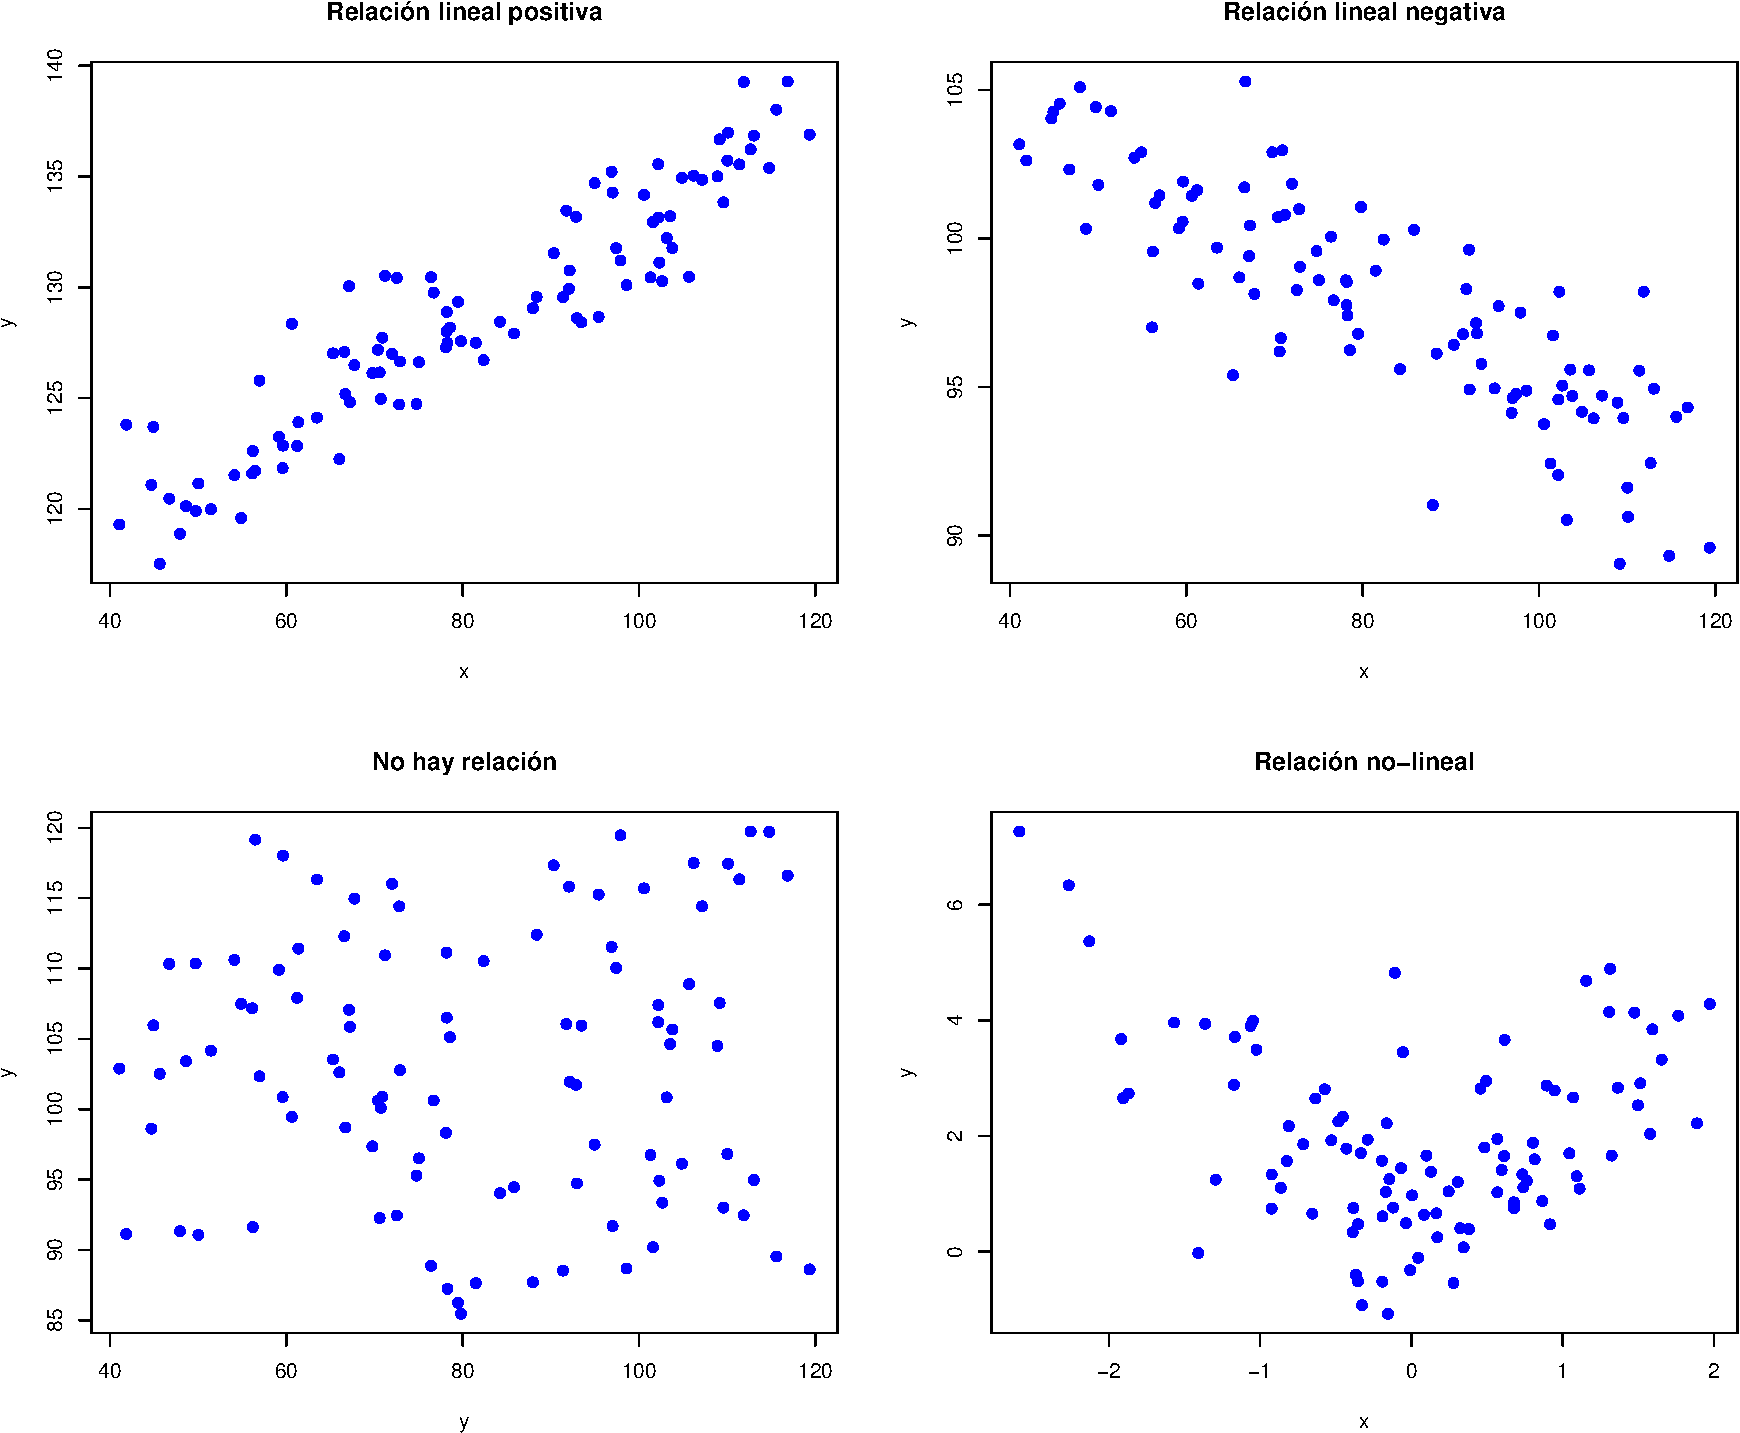
\includegraphics{tema8_files/figure-latex/unnamed-chunk-3-1.pdf}

Matriz de correlaciones

\begin{Shaded}
\begin{Highlighting}[]
\KeywordTok{round}\NormalTok{(}\KeywordTok{cor}\NormalTok{(heptathlon[,-score]),}\DecValTok{3}\NormalTok{)}
\end{Highlighting}
\end{Shaded}

\begin{verbatim}
##          hurdles highjump  shot run200m longjump javelin run800m
## hurdles    1.000    0.811 0.651   0.774    0.912   0.008   0.779
## highjump   0.811    1.000 0.441   0.488    0.782   0.002   0.591
## shot       0.651    0.441 1.000   0.683    0.743   0.269   0.420
## run200m    0.774    0.488 0.683   1.000    0.817   0.333   0.617
## longjump   0.912    0.782 0.743   0.817    1.000   0.067   0.700
## javelin    0.008    0.002 0.269   0.333    0.067   1.000  -0.020
## run800m    0.779    0.591 0.420   0.617    0.700  -0.020   1.000
\end{verbatim}

el resultado confirma que la gran mayoría de las correlaciones entre las
pruebas son positivas, con una correlación alta entre el salto de
longitud (\texttt{longjump}) y los 100m vallas (\texttt{hurdles}).
Algunos menos como el salto de altura (\texttt{highjump}) y el
lanzamiento de peso (\texttt{shot}) y la jabalina (\texttt{javelin}) que
presenta una correlación cercana a cero con el resto de pruebas.

Una posible expliación a este resultado puede deberse a que el
entrenamiento para las otras 6 pruebas, no aporta demasiado al de la
prueba de jabalina, que es una prueba más técnica.

Se puede observar que hay un valor atípico en casi todas las pruebas que
corresponde a una atleta \texttt{Launa\ (PNG)} de Papua Nueva Guinea-
Eliminaremos esta observación para ver si la matriz de correlaciones es
sensiblemente distinta:

\begin{Shaded}
\begin{Highlighting}[]
\NormalTok{heptathlon <-}\StringTok{ }\NormalTok{heptathlon[-}\KeywordTok{which}\NormalTok{(}\KeywordTok{rownames}\NormalTok{(heptathlon)==}\StringTok{"Launa (PNG)"}\NormalTok{),]}
\KeywordTok{plot}\NormalTok{(heptathlon[,-score])}
\end{Highlighting}
\end{Shaded}

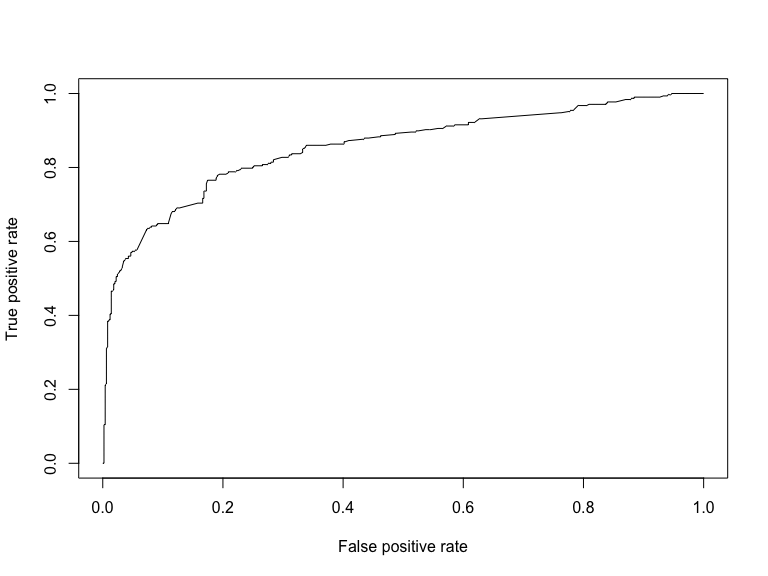
\includegraphics{tema8_files/figure-latex/unnamed-chunk-5-1.pdf}

Eliminando a la atleta de Papua Nueva Guinea, las correlaciones cambian
sustancialmente y en el diagrama de dispersión de la matriz, no se
observan valores extremos.

\begin{Shaded}
\begin{Highlighting}[]
\KeywordTok{round}\NormalTok{(}\KeywordTok{cor}\NormalTok{(heptathlon[,-score]),}\DecValTok{3}\NormalTok{)}
\end{Highlighting}
\end{Shaded}

\begin{verbatim}
##          hurdles highjump  shot run200m longjump javelin run800m
## hurdles    1.000    0.582 0.767   0.830    0.889   0.332   0.559
## highjump   0.582    1.000 0.465   0.391    0.663   0.348   0.152
## shot       0.767    0.465 1.000   0.669    0.784   0.343   0.408
## run200m    0.830    0.391 0.669   1.000    0.811   0.471   0.573
## longjump   0.889    0.663 0.784   0.811    1.000   0.287   0.523
## javelin    0.332    0.348 0.343   0.471    0.287   1.000   0.256
## run800m    0.559    0.152 0.408   0.573    0.523   0.256   1.000
\end{verbatim}

Para realizar el PCA, partiremos de la matriz de correlaciones, ya que
las 7 pruebas están medidas en diferentes escalas (metros, segundos). A
este procedimiento se le denomina PCA normalizado (\texttt{scale=TRUE}
en la función \texttt{prcomp}).

\begin{Shaded}
\begin{Highlighting}[]
\NormalTok{?prcomp}
\NormalTok{heptathlon_pca <-}\StringTok{ }\KeywordTok{prcomp}\NormalTok{(heptathlon[,-score],}\DataTypeTok{scale=}\OtherTok{TRUE}\NormalTok{)}
\KeywordTok{head}\NormalTok{(heptathlon_pca)}
\end{Highlighting}
\end{Shaded}

\begin{verbatim}
## $sdev
## [1] 2.0793370 0.9481532 0.9109016 0.6831967 0.5461888 0.3374549 0.2620420
## 
## $rotation
##                 PC1         PC2        PC3         PC4         PC5
## hurdles  -0.4503876  0.05772161 -0.1739345  0.04840598 -0.19889364
## highjump -0.3145115 -0.65133162 -0.2088272 -0.55694554  0.07076358
## shot     -0.4024884 -0.02202088 -0.1534709  0.54826705  0.67166466
## run200m  -0.4270860  0.18502783  0.1301287  0.23095946 -0.61781764
## longjump -0.4509639 -0.02492486 -0.2697589 -0.01468275 -0.12151793
## javelin  -0.2423079 -0.32572229  0.8806995  0.06024757  0.07874396
## run800m  -0.3029068  0.65650503  0.1930020 -0.57418128  0.31880178
##                  PC6         PC7
## hurdles   0.84665086 -0.06961672
## highjump -0.09007544  0.33155910
## shot     -0.09886359  0.22904298
## run200m  -0.33279359  0.46971934
## longjump -0.38294411 -0.74940781
## javelin   0.07193437 -0.21108138
## run800m  -0.05217664  0.07718616
## 
## $center
##   hurdles  highjump      shot   run200m  longjump   javelin   run800m 
##  2.687500  1.793750 13.173333  2.023750  6.205417 41.278333 28.516667 
## 
## $scale
##    hurdles   highjump       shot    run200m   longjump    javelin 
## 0.51456398 0.05232112 1.49714995 0.93676972 0.40165938 3.46870690 
##    run800m 
## 6.14724800 
## 
## $x
##                              PC1         PC2          PC3          PC4
## Joyner-Kersee (USA) -4.757530189 -0.13986143 -0.006040526  0.293416339
## John (GDR)          -3.147943402  0.94859029 -0.243919842  0.549171385
## Behmer (GDR)        -2.926184760  0.69534239  0.622293440 -0.554744912
## Sablovskaite (URS)  -1.288135516  0.17900713  0.250632380  0.637174187
## Choubenkova (URS)   -1.503450994  0.96177329  1.780588549  0.784035325
## Schulz (GDR)        -0.958467101  0.35121643  0.413086366 -1.113546938
## Fleming (AUS)       -0.953445060  0.49982537 -0.265135015 -0.140202490
## Greiner (USA)       -0.633239267  0.37592917 -1.140338594  0.142558348
## Lajbnerova (CZE)    -0.381571974 -0.71213459 -0.068395353  0.087212735
## Bouraga (URS)       -0.522322004  0.77688861 -0.481071429  0.283745698
## Wijnsma (HOL)       -0.217701500 -0.23369645 -1.154221444 -1.260128609
## Dimitrova (BUL)     -1.075984276  0.51552998 -0.312458252 -0.127032432
## Scheider (SWI)       0.003014986 -1.44688825  1.582739069 -1.254415325
## Braun (FRG)          0.109183759 -1.63595645  0.469577294  0.362580442
## Ruotsalainen (FIN)   0.208868056 -0.68866173  1.152140223 -0.112914470
## Yuping (CHN)         0.232507119 -1.95999641 -1.541230813  0.598325122
## Hagger (GB)          0.659520046 -0.08775813 -1.796509771 -0.182375000
## Brown (USA)          0.756854602 -2.04292201  0.451506018  0.476926314
## Mulliner (GB)        1.880932819  0.91530324 -0.359311801  0.799619094
## Hautenauve (BEL)     1.828170404  0.72629699 -1.048640439 -0.711793161
## Kytola (FIN)         2.118203163  0.39921397  0.190158154 -0.788445056
## Geremias (BRA)       2.770706272  0.03463584  0.170274969  1.385562494
## Hui-Ing (TAI)        3.901166920  1.20175472  0.943677497 -0.002429122
## Jeong-Mi (KOR)       3.896847898  0.36656804  0.390599321 -0.152299968
##                             PC5         PC6         PC7
## Joyner-Kersee (USA) -0.36183307 -0.27050283 -0.47587527
## John (GDR)           0.75364464  0.37770017 -0.05172711
## Behmer (GDR)        -0.19035037 -0.25780287  0.11054960
## Sablovskaite (URS)   0.60362153 -0.21575716  0.53075152
## Choubenkova (URS)    0.58969949  0.08014332 -0.30081842
## Schulz (GDR)         0.71483887 -0.25436956  0.03838796
## Fleming (AUS)       -0.86581530  0.03691813  0.23005943
## Greiner (USA)        0.20807431 -0.14236240 -0.06374657
## Lajbnerova (CZE)     0.67727618  0.25014881  0.35555639
## Bouraga (URS)       -1.18784299  0.39881271  0.19712215
## Wijnsma (HOL)        0.37497195 -0.20267731  0.17459647
## Dimitrova (BUL)     -0.91992929  0.26727067  0.21111846
## Scheider (SWI)      -0.20526249  0.17597425 -0.03915701
## Braun (FRG)         -0.14712208  0.26134199 -0.01334416
## Ruotsalainen (FIN)  -0.31539746  0.18351622 -0.14127555
## Yuping (CHN)         0.17451428 -0.50175724  0.04999374
## Hagger (GB)         -0.05104049  0.55058471 -0.46388534
## Brown (USA)         -0.38154294 -0.26606429 -0.11099445
## Mulliner (GB)       -0.06942955 -0.73259727 -0.31281502
## Hautenauve (BEL)     0.14092347  0.06933542 -0.07548638
## Kytola (FIN)         0.41815113 -0.03363651  0.12143219
## Geremias (BRA)       0.28541366  0.38083979  0.34574480
## Hui-Ing (TAI)       -0.67080776 -0.52756760  0.09436975
## Jeong-Mi (KOR)       0.42524426  0.37250885 -0.41055719
\end{verbatim}

\begin{Shaded}
\begin{Highlighting}[]
\NormalTok{a1 <-}\StringTok{ }\NormalTok{heptathlon_pca$rotation[,}\DecValTok{1}\NormalTok{]}
\end{Highlighting}
\end{Shaded}

Podemos resumir el análisis con \texttt{summary}

\begin{Shaded}
\begin{Highlighting}[]
\KeywordTok{summary}\NormalTok{(heptathlon_pca)}
\end{Highlighting}
\end{Shaded}

\begin{verbatim}
## Importance of components:
##                           PC1    PC2    PC3     PC4     PC5     PC6
## Standard deviation     2.0793 0.9482 0.9109 0.68320 0.54619 0.33745
## Proportion of Variance 0.6177 0.1284 0.1185 0.06668 0.04262 0.01627
## Cumulative Proportion  0.6177 0.7461 0.8646 0.93131 0.97392 0.99019
##                            PC7
## Standard deviation     0.26204
## Proportion of Variance 0.00981
## Cumulative Proportion  1.00000
\end{verbatim}

Los primeros 2 componentes explican un 75\% de la varianza explicada y
las 3 primeras un 86\%.

\begin{Shaded}
\begin{Highlighting}[]
\KeywordTok{head}\NormalTok{(heptathlon_pca$x)}
\end{Highlighting}
\end{Shaded}

\begin{verbatim}
##                            PC1        PC2          PC3        PC4
## Joyner-Kersee (USA) -4.7575302 -0.1398614 -0.006040526  0.2934163
## John (GDR)          -3.1479434  0.9485903 -0.243919842  0.5491714
## Behmer (GDR)        -2.9261848  0.6953424  0.622293440 -0.5547449
## Sablovskaite (URS)  -1.2881355  0.1790071  0.250632380  0.6371742
## Choubenkova (URS)   -1.5034510  0.9617733  1.780588549  0.7840353
## Schulz (GDR)        -0.9584671  0.3512164  0.413086366 -1.1135469
##                            PC5         PC6         PC7
## Joyner-Kersee (USA) -0.3618331 -0.27050283 -0.47587527
## John (GDR)           0.7536446  0.37770017 -0.05172711
## Behmer (GDR)        -0.1903504 -0.25780287  0.11054960
## Sablovskaite (URS)   0.6036215 -0.21575716  0.53075152
## Choubenkova (URS)    0.5896995  0.08014332 -0.30081842
## Schulz (GDR)         0.7148389 -0.25436956  0.03838796
\end{verbatim}

Graficamente, se observa que la primera componente principal es la más
dominante.

\begin{Shaded}
\begin{Highlighting}[]
\KeywordTok{plot}\NormalTok{(heptathlon_pca)}
\end{Highlighting}
\end{Shaded}

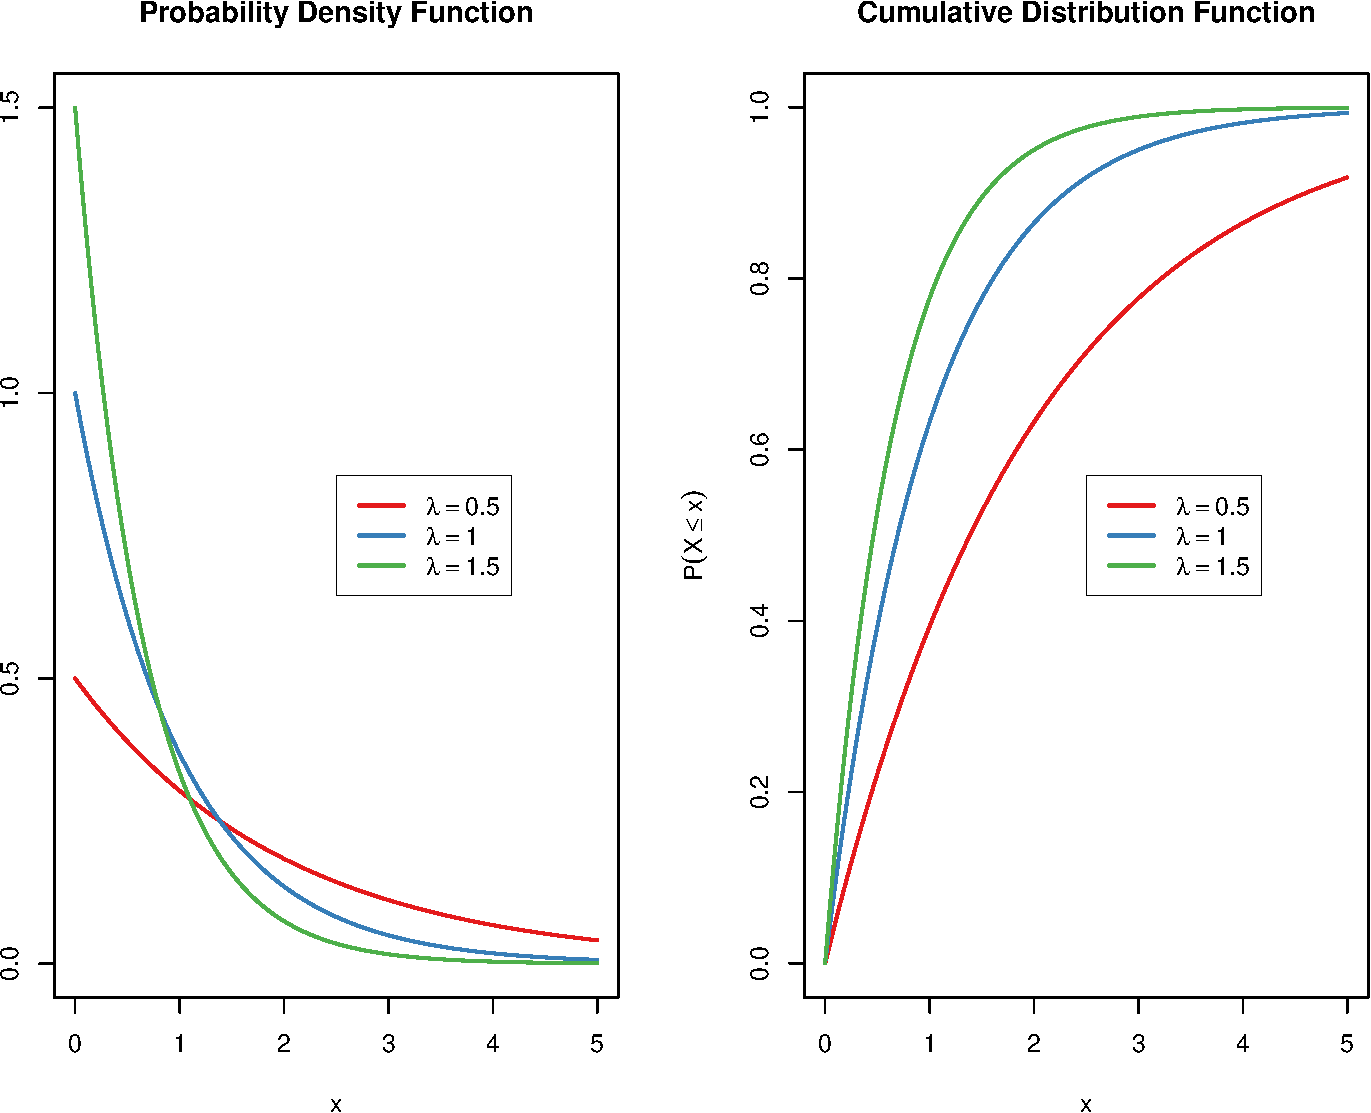
\includegraphics{tema8_files/figure-latex/unnamed-chunk-10-1.pdf}

El \emph{biplot} es una representación gráfica de datos multivariantes.
De la misma manera que un diagrama de dispersión muestra la distribución
conjunta de dos variables, un \textbf{biplot} representa tres o más
variables.

Si ordenamos de mayor a menor la variable \texttt{score} tenemos a las
tres medallas de oro, plata y bronce.

\begin{Shaded}
\begin{Highlighting}[]
\KeywordTok{head}\NormalTok{(heptathlon[}\KeywordTok{order}\NormalTok{(heptathlon$score,}\DataTypeTok{decreasing =} \OtherTok{TRUE}\NormalTok{),],}\DecValTok{3}\NormalTok{)}
\end{Highlighting}
\end{Shaded}

\begin{verbatim}
##                     hurdles highjump  shot run200m longjump javelin
## Joyner-Kersee (USA)    3.73     1.86 15.80    4.05     7.27   45.66
## John (GDR)             3.57     1.80 16.23    2.96     6.71   42.56
## Behmer (GDR)           3.22     1.83 14.20    3.51     6.68   44.54
##                     run800m score
## Joyner-Kersee (USA)   34.92  7291
## John (GDR)            37.31  6897
## Behmer (GDR)          39.23  6858
\end{verbatim}

El biplot, nos muestra a las atletas proyectadas sobres sus 2 primeras
componentes principales, pero además las flechas nos dan información de
las varianzas y covarianzas de las variables (direcciones de máxima
variabilidad).

\begin{Shaded}
\begin{Highlighting}[]
\KeywordTok{biplot}\NormalTok{(heptathlon_pca)}
\end{Highlighting}
\end{Shaded}

\begin{center}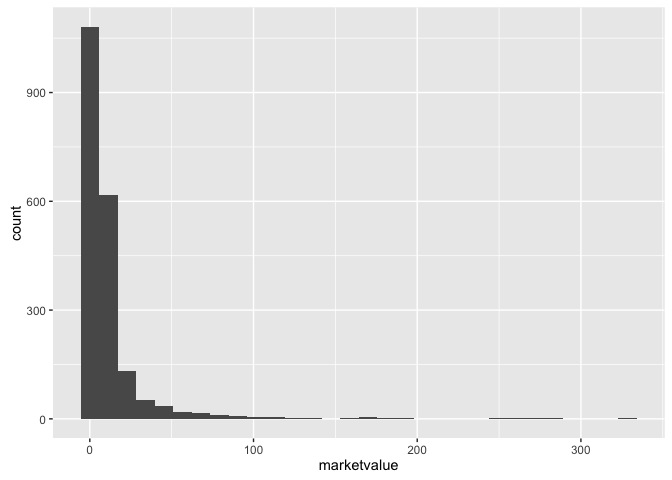
\includegraphics{tema8_files/figure-latex/unnamed-chunk-12-1} \end{center}

Por ejemplo, la ganadora de la prueba \texttt{Joyner-Kersee\ (USA)}
acumula mayores puntuaciones en las pruebas \texttt{longjump},
\texttt{hurdles} y \texttt{run200m}.

Podemos analizar la correlación entre la variable \texttt{score} y la
PC1. Lo cual indica que la correlación es muy negativa y muy fuerte con
el \texttt{score}.

\begin{Shaded}
\begin{Highlighting}[]
\KeywordTok{cor}\NormalTok{(heptathlon$score, heptathlon_pca$x[,}\DecValTok{1}\NormalTok{])}
\end{Highlighting}
\end{Shaded}

\begin{verbatim}
## [1] -0.9931168
\end{verbatim}

\begin{Shaded}
\begin{Highlighting}[]
\KeywordTok{plot}\NormalTok{(heptathlon$score, heptathlon_pca$x[,}\DecValTok{1}\NormalTok{])}
\end{Highlighting}
\end{Shaded}

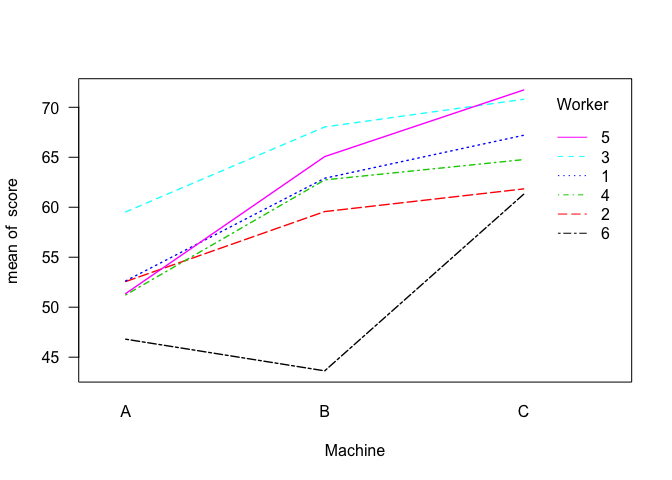
\includegraphics{tema8_files/figure-latex/unnamed-chunk-13-1.pdf}

Los objetos de la funcion \texttt{prcomp}

\begin{Shaded}
\begin{Highlighting}[]
\KeywordTok{class}\NormalTok{(heptathlon_pca)}
\end{Highlighting}
\end{Shaded}

\begin{verbatim}
## [1] "prcomp"
\end{verbatim}

permiten utilizar la funcion \texttt{predict}. Por ejemplo:

\begin{Shaded}
\begin{Highlighting}[]
\NormalTok{new.athlete <-}\StringTok{ }\KeywordTok{as.data.frame}\NormalTok{(}\KeywordTok{t}\NormalTok{(}\KeywordTok{as.vector}\NormalTok{(}\KeywordTok{c}\NormalTok{(}\FloatTok{3.5}\NormalTok{,}\DecValTok{2}\NormalTok{,}\DecValTok{13}\NormalTok{,}\DecValTok{5}\NormalTok{,}\DecValTok{7}\NormalTok{,}\DecValTok{41}\NormalTok{,}\DecValTok{33}\NormalTok{))))}
\KeywordTok{colnames}\NormalTok{(new.athlete) <-}\StringTok{ }\KeywordTok{c}\NormalTok{(}\StringTok{"hurdles"}\NormalTok{,}\StringTok{"highjump"}\NormalTok{,}
                           \StringTok{"shot"}\NormalTok{,}\StringTok{"run200m"}\NormalTok{,}\StringTok{"longjump"}\NormalTok{,}
                           \StringTok{"javelin"}\NormalTok{,}\StringTok{"run800m"}\NormalTok{)}
\KeywordTok{rownames}\NormalTok{(new.athlete) <-}\StringTok{ "Mrs XYZ (XXX)"}
\NormalTok{pp<-}\KeywordTok{predict}\NormalTok{(heptathlon_pca,}\DataTypeTok{newdata =} \NormalTok{new.athlete)}
\NormalTok{pp}
\end{Highlighting}
\end{Shaded}

\begin{verbatim}
##                     PC1       PC2       PC3       PC4       PC5        PC6
## Mrs XYZ (XXX) -4.354879 -1.430366 -1.130194 -1.901377 -2.089963 -0.8654821
##                    PC7
## Mrs XYZ (XXX) 1.253643
\end{verbatim}

\begin{Shaded}
\begin{Highlighting}[]
\KeywordTok{biplot}\NormalTok{(heptathlon_pca)}
\KeywordTok{text}\NormalTok{(pp[,}\DecValTok{1}\NormalTok{],pp[,}\DecValTok{2}\NormalTok{],}\StringTok{"Mrs XYZ (XXX)"}\NormalTok{,}\DataTypeTok{col=}\StringTok{"blue"}\NormalTok{,}\DataTypeTok{cex=}\NormalTok{.}\DecValTok{65}\NormalTok{)}
\end{Highlighting}
\end{Shaded}

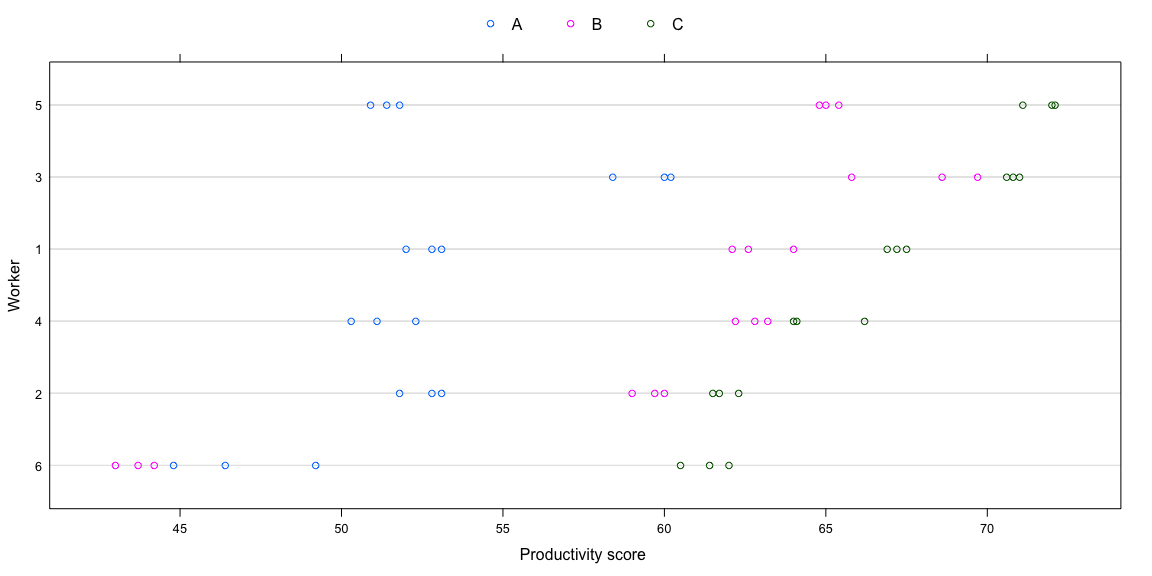
\includegraphics{tema8_files/figure-latex/unnamed-chunk-15-1.pdf}

\subsubsection{Regresion y PCA}\label{regresion-y-pca}

Volvamos al ejemplo \texttt{housing,data}. Vamos a tratar de predecir el
valor medio de las casas ocupadas por sus dueños en miles de dólares
(MEDV) usando las tres primeras PCs de un PCA.

\begin{Shaded}
\begin{Highlighting}[]
\NormalTok{houses <-}\StringTok{ }\KeywordTok{read.table}\NormalTok{(}\StringTok{"http://archive.ics.uci.edu/ml/machine-learning-databases/housing/housing.data"}\NormalTok{,}
                     \DataTypeTok{header =} \NormalTok{F, }\DataTypeTok{na.string =} \StringTok{"?"}\NormalTok{)}
\KeywordTok{colnames}\NormalTok{(houses) <-}\StringTok{ }\KeywordTok{c}\NormalTok{(}\StringTok{"CRIM"}\NormalTok{, }\StringTok{"ZN"}\NormalTok{, }\StringTok{"INDUS"}\NormalTok{,}\StringTok{"CHAS"}\NormalTok{,}
                      \StringTok{"NOX"}\NormalTok{,}\StringTok{"RM"}\NormalTok{,}\StringTok{"AGE"}\NormalTok{,}\StringTok{"DIS"}\NormalTok{,}\StringTok{"RAD"}\NormalTok{,}
                      \StringTok{"TAX"}\NormalTok{,}\StringTok{"PTRATIO"}\NormalTok{,}\StringTok{"B"}\NormalTok{,}\StringTok{"LSTAT"}\NormalTok{,}\StringTok{"MEDV"}\NormalTok{)}

\CommentTok{# Perform PCA}
\NormalTok{pcaHouses <-}\StringTok{ }\KeywordTok{prcomp}\NormalTok{(houses[,-}\DecValTok{14}\NormalTok{],}\DataTypeTok{scale=}\OtherTok{TRUE}\NormalTok{)}

\KeywordTok{summary}\NormalTok{(pcaHouses)}
\end{Highlighting}
\end{Shaded}

\begin{verbatim}
## Importance of components:
##                           PC1    PC2     PC3     PC4     PC5     PC6
## Standard deviation     2.4752 1.1972 1.11473 0.92605 0.91368 0.81081
## Proportion of Variance 0.4713 0.1103 0.09559 0.06597 0.06422 0.05057
## Cumulative Proportion  0.4713 0.5816 0.67713 0.74310 0.80732 0.85789
##                            PC7     PC8    PC9    PC10    PC11    PC12
## Standard deviation     0.73168 0.62936 0.5263 0.46930 0.43129 0.41146
## Proportion of Variance 0.04118 0.03047 0.0213 0.01694 0.01431 0.01302
## Cumulative Proportion  0.89907 0.92954 0.9508 0.96778 0.98209 0.99511
##                           PC13
## Standard deviation     0.25201
## Proportion of Variance 0.00489
## Cumulative Proportion  1.00000
\end{verbatim}

\begin{Shaded}
\begin{Highlighting}[]
\NormalTok{scoresHouses <-}\StringTok{ }\NormalTok{pcaHouses$x}
 
\CommentTok{# Fit lm using the first 3 PCs}
\NormalTok{modHouses <-}\StringTok{ }\KeywordTok{lm}\NormalTok{(houses$MEDV ~}\StringTok{ }\NormalTok{scoresHouses[,}\DecValTok{1}\NormalTok{:}\DecValTok{3}\NormalTok{])}
\KeywordTok{summary}\NormalTok{(modHouses)}
\end{Highlighting}
\end{Shaded}

\begin{verbatim}
## 
## Call:
## lm(formula = houses$MEDV ~ scoresHouses[, 1:3])
## 
## Residuals:
##     Min      1Q  Median      3Q     Max 
## -16.774  -3.082  -0.651   2.091  35.000 
## 
## Coefficients:
##                        Estimate Std. Error t value Pr(>|t|)    
## (Intercept)             22.5328     0.2474   91.06   <2e-16 ***
## scoresHouses[, 1:3]PC1  -2.2730     0.1001  -22.72   <2e-16 ***
## scoresHouses[, 1:3]PC2   2.1949     0.2069   10.61   <2e-16 ***
## scoresHouses[, 1:3]PC3   3.5010     0.2222   15.76   <2e-16 ***
## ---
## Signif. codes:  0 '***' 0.001 '**' 0.01 '*' 0.05 '.' 0.1 ' ' 1
## 
## Residual standard error: 5.566 on 502 degrees of freedom
## Multiple R-squared:  0.6359, Adjusted R-squared:  0.6337 
## F-statistic: 292.3 on 3 and 502 DF,  p-value: < 2.2e-16
\end{verbatim}

Comparamos con el modelo lineal con todas las variables

\begin{Shaded}
\begin{Highlighting}[]
\CommentTok{# Fit lm using all 14 vars}
\NormalTok{modHousesFull <-}\StringTok{ }\KeywordTok{lm}\NormalTok{(MEDV ~}\StringTok{ }\NormalTok{., }\DataTypeTok{data =} \NormalTok{houses)}
\KeywordTok{summary}\NormalTok{(modHousesFull) }\CommentTok{# R2 = 0.741}
\end{Highlighting}
\end{Shaded}

\begin{verbatim}
## 
## Call:
## lm(formula = MEDV ~ ., data = houses)
## 
## Residuals:
##     Min      1Q  Median      3Q     Max 
## -15.595  -2.730  -0.518   1.777  26.199 
## 
## Coefficients:
##               Estimate Std. Error t value Pr(>|t|)    
## (Intercept)  3.646e+01  5.103e+00   7.144 3.28e-12 ***
## CRIM        -1.080e-01  3.286e-02  -3.287 0.001087 ** 
## ZN           4.642e-02  1.373e-02   3.382 0.000778 ***
## INDUS        2.056e-02  6.150e-02   0.334 0.738288    
## CHAS         2.687e+00  8.616e-01   3.118 0.001925 ** 
## NOX         -1.777e+01  3.820e+00  -4.651 4.25e-06 ***
## RM           3.810e+00  4.179e-01   9.116  < 2e-16 ***
## AGE          6.922e-04  1.321e-02   0.052 0.958229    
## DIS         -1.476e+00  1.995e-01  -7.398 6.01e-13 ***
## RAD          3.060e-01  6.635e-02   4.613 5.07e-06 ***
## TAX         -1.233e-02  3.760e-03  -3.280 0.001112 ** 
## PTRATIO     -9.527e-01  1.308e-01  -7.283 1.31e-12 ***
## B            9.312e-03  2.686e-03   3.467 0.000573 ***
## LSTAT       -5.248e-01  5.072e-02 -10.347  < 2e-16 ***
## ---
## Signif. codes:  0 '***' 0.001 '**' 0.01 '*' 0.05 '.' 0.1 ' ' 1
## 
## Residual standard error: 4.745 on 492 degrees of freedom
## Multiple R-squared:  0.7406, Adjusted R-squared:  0.7338 
## F-statistic: 108.1 on 13 and 492 DF,  p-value: < 2.2e-16
\end{verbatim}

\begin{Shaded}
\begin{Highlighting}[]
\CommentTok{# Compare obs. vs. pred. plots}
\KeywordTok{par}\NormalTok{(}\DataTypeTok{mfrow =} \KeywordTok{c}\NormalTok{(}\DecValTok{1}\NormalTok{,}\DecValTok{2}\NormalTok{))}
\KeywordTok{plot}\NormalTok{(houses$MEDV, }\KeywordTok{predict}\NormalTok{(modHouses), }
     \DataTypeTok{xlab =} \StringTok{"Observed MEDV"}\NormalTok{, }\DataTypeTok{ylab =} \StringTok{"Predicted MEDV"}\NormalTok{, }\DataTypeTok{main =} \StringTok{"PCR"}\NormalTok{, }\KeywordTok{abline}\NormalTok{(}\DataTypeTok{a =} \DecValTok{0}\NormalTok{, }\DataTypeTok{b =} \DecValTok{1}\NormalTok{, }\DataTypeTok{col =} \StringTok{"red"}\NormalTok{))}
\KeywordTok{plot}\NormalTok{(houses$MEDV, }\KeywordTok{predict}\NormalTok{(modHousesFull),}
     \DataTypeTok{xlab =} \StringTok{"Observed MEDV"}\NormalTok{, }\DataTypeTok{ylab =} \StringTok{"Predicted MEDV"}\NormalTok{, }\DataTypeTok{main =} \StringTok{"Full model"}\NormalTok{, }\KeywordTok{abline}\NormalTok{(}\DataTypeTok{a =} \DecValTok{0}\NormalTok{, }\DataTypeTok{b =} \DecValTok{1}\NormalTok{, }\DataTypeTok{col =} \StringTok{"red"}\NormalTok{))}
\end{Highlighting}
\end{Shaded}

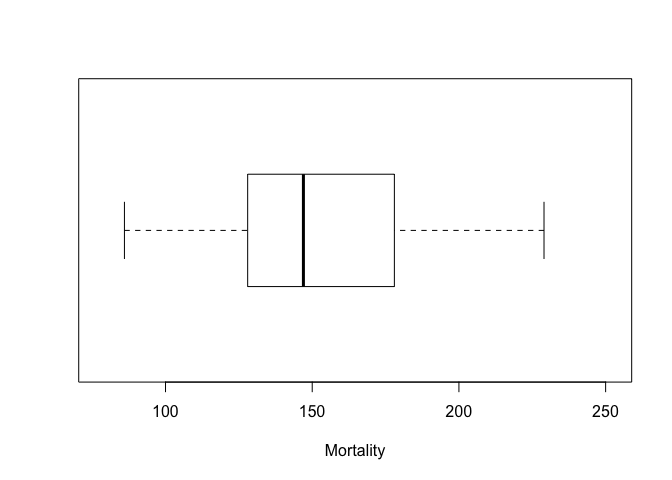
\includegraphics{tema8_files/figure-latex/unnamed-chunk-17-1.pdf}

\textbf{Ejemplo}

\begin{Shaded}
\begin{Highlighting}[]
\KeywordTok{data}\NormalTok{(USArrests)}
\KeywordTok{head}\NormalTok{(USArrests)}
\end{Highlighting}
\end{Shaded}

\begin{verbatim}
##            Murder Assault UrbanPop Rape
## Alabama      13.2     236       58 21.2
## Alaska       10.0     263       48 44.5
## Arizona       8.1     294       80 31.0
## Arkansas      8.8     190       50 19.5
## California    9.0     276       91 40.6
## Colorado      7.9     204       78 38.7
\end{verbatim}

\begin{Shaded}
\begin{Highlighting}[]
\CommentTok{# PCA with function prcomp}
\NormalTok{pca1 =}\StringTok{ }\KeywordTok{prcomp}\NormalTok{(USArrests, }\DataTypeTok{scale. =} \OtherTok{TRUE}\NormalTok{)}

\CommentTok{# sqrt of eigenvalues}
\NormalTok{pca1$sdev}
\end{Highlighting}
\end{Shaded}

\begin{verbatim}
## [1] 1.5748783 0.9948694 0.5971291 0.4164494
\end{verbatim}

\begin{Shaded}
\begin{Highlighting}[]
\CommentTok{# loadings}
\KeywordTok{head}\NormalTok{(pca1$rotation)}
\end{Highlighting}
\end{Shaded}

\begin{verbatim}
##                 PC1        PC2        PC3         PC4
## Murder   -0.5358995  0.4181809 -0.3412327  0.64922780
## Assault  -0.5831836  0.1879856 -0.2681484 -0.74340748
## UrbanPop -0.2781909 -0.8728062 -0.3780158  0.13387773
## Rape     -0.5434321 -0.1673186  0.8177779  0.08902432
\end{verbatim}

\begin{Shaded}
\begin{Highlighting}[]
\CommentTok{# PCs (aka scores)}
\KeywordTok{head}\NormalTok{(pca1$x)}
\end{Highlighting}
\end{Shaded}

\begin{verbatim}
##                   PC1        PC2         PC3          PC4
## Alabama    -0.9756604  1.1220012 -0.43980366  0.154696581
## Alaska     -1.9305379  1.0624269  2.01950027 -0.434175454
## Arizona    -1.7454429 -0.7384595  0.05423025 -0.826264240
## Arkansas    0.1399989  1.1085423  0.11342217 -0.180973554
## California -2.4986128 -1.5274267  0.59254100 -0.338559240
## Colorado   -1.4993407 -0.9776297  1.08400162  0.001450164
\end{verbatim}

\begin{Shaded}
\begin{Highlighting}[]
\KeywordTok{plot}\NormalTok{(pca1)}
\end{Highlighting}
\end{Shaded}

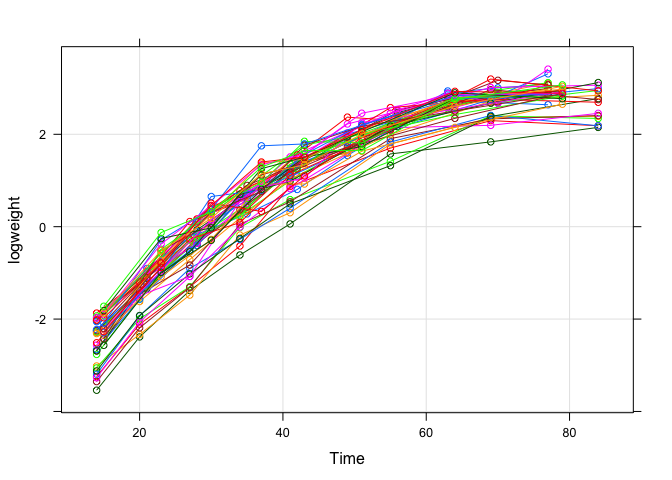
\includegraphics{tema8_files/figure-latex/unnamed-chunk-19-1.pdf}

\begin{Shaded}
\begin{Highlighting}[]
\KeywordTok{biplot}\NormalTok{(pca1)}
\end{Highlighting}
\end{Shaded}

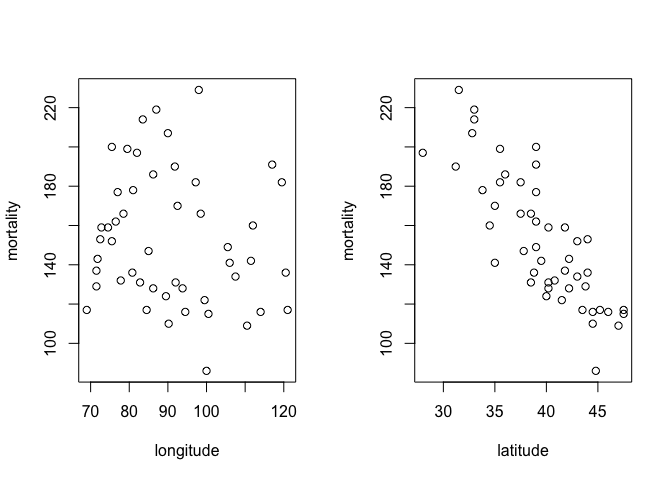
\includegraphics{tema8_files/figure-latex/unnamed-chunk-20-1.pdf}

Podemos cambiar el eje

\begin{Shaded}
\begin{Highlighting}[]
\NormalTok{pca.out <-}\StringTok{ }\NormalTok{pca1}
\NormalTok{pca.out$rotation <-}\StringTok{ }\NormalTok{-pca.out$rotation}
\NormalTok{pca.out$x <-}\StringTok{ }\NormalTok{-pca.out$x}
\KeywordTok{biplot}\NormalTok{(pca.out,}\DataTypeTok{scale=}\DecValTok{0}\NormalTok{, }\DataTypeTok{cex=}\NormalTok{.}\DecValTok{7}\NormalTok{)}
\end{Highlighting}
\end{Shaded}

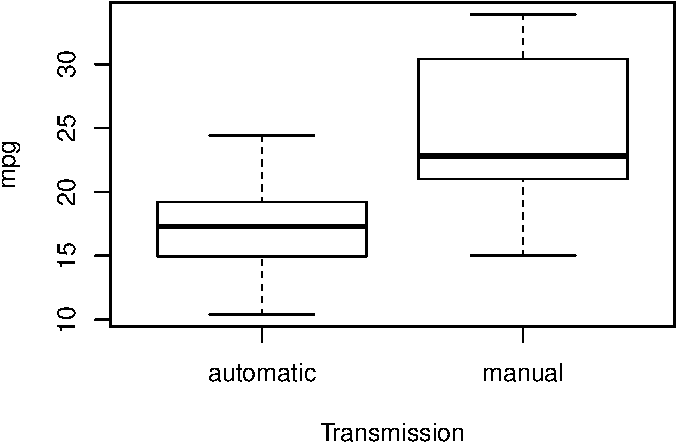
\includegraphics{tema8_files/figure-latex/unnamed-chunk-21-1.pdf}

\textbf{Interpretación del biplot:} Para cada una de los 50 estados en
los Estados Unidos, el conjunto de datos contiene el número de arrestos
por cada 100.000 residentes por cada tres crímenes: Asalto, Asesinato y
Violación. También \texttt{Urbanpop} representa el porcentaje de la
población en cada estado que vive en áreas urbanas. La gráfica muestra
las dos primeras puntuaciones de los componentes principales y el vector
\texttt{loading}s en gráfico simple.

\begin{Shaded}
\begin{Highlighting}[]
\NormalTok{pca.out$rotation[,}\DecValTok{1}\NormalTok{:}\DecValTok{2}\NormalTok{]}
\end{Highlighting}
\end{Shaded}

\begin{verbatim}
##                PC1        PC2
## Murder   0.5358995 -0.4181809
## Assault  0.5831836 -0.1879856
## UrbanPop 0.2781909  0.8728062
## Rape     0.5434321  0.1673186
\end{verbatim}

El PC1, muestra como el peso de las variables \texttt{Murder},
\texttt{Assault} y \texttt{Rape} es similar, y más pequeño para
\texttt{UrbanPop}. Por lo tanto, este componente corresponde
aproximadamente a una medida de las tasas globales de delitos graves.

El PC2, tiene un peso mucho mayor en \texttt{Urbanpop}, y mucho menor en
el resto. Por lo tanto, este componente corresponde aproximadamente al
nivel de urbanización del estado.

En general, vemos que las variables relacionadas con el delito están
situadas cerca unas de otras, y que la variable urbanpop está lejos de
las otras tres. Esto indica que las variables relacionadas con el delito
están correlacionadas entre sí. Los estados con altas tasas de homicidio
tienden a tener altas tasas de agresión y violación. La variable
\texttt{Urbanpop} está menos correlacionada con las otras tres. Otro
paquete de \texttt{R} es \texttt{FactorMineR}

\begin{Shaded}
\begin{Highlighting}[]
\CommentTok{# PCA with function PCA}
\KeywordTok{library}\NormalTok{(FactoMineR)}
\end{Highlighting}
\end{Shaded}

\begin{verbatim}
## Warning: package 'FactoMineR' was built under R version 3.3.2
\end{verbatim}

\begin{Shaded}
\begin{Highlighting}[]
\CommentTok{# apply PCA}
\NormalTok{pca3 =}\StringTok{ }\KeywordTok{PCA}\NormalTok{(USArrests, }\DataTypeTok{graph =} \OtherTok{FALSE}\NormalTok{)}

\CommentTok{# matrix with eigenvalues}
\NormalTok{pca3$eig}
\end{Highlighting}
\end{Shaded}

\begin{verbatim}
##        eigenvalue percentage of variance cumulative percentage of variance
## comp 1  2.4802416              62.006039                          62.00604
## comp 2  0.9897652              24.744129                          86.75017
## comp 3  0.3565632               8.914080                          95.66425
## comp 4  0.1734301               4.335752                         100.00000
\end{verbatim}

\begin{Shaded}
\begin{Highlighting}[]
\CommentTok{# correlations between variables and PCs}
\NormalTok{pca3$var$coord}
\end{Highlighting}
\end{Shaded}

\begin{verbatim}
##              Dim.1      Dim.2      Dim.3       Dim.4
## Murder   0.8439764 -0.4160354  0.2037600  0.27037052
## Assault  0.9184432 -0.1870211  0.1601192 -0.30959159
## UrbanPop 0.4381168  0.8683282  0.2257242  0.05575330
## Rape     0.8558394  0.1664602 -0.4883190  0.03707412
\end{verbatim}

\begin{Shaded}
\begin{Highlighting}[]
\KeywordTok{plot}\NormalTok{(pca3)}
\end{Highlighting}
\end{Shaded}

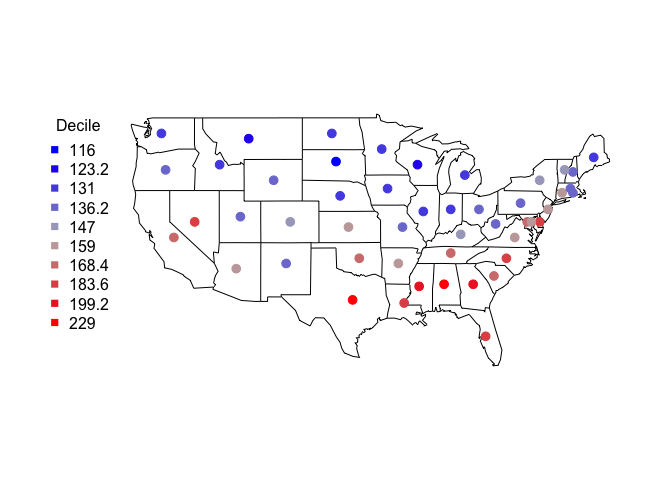
\includegraphics{tema8_files/figure-latex/unnamed-chunk-23-1.pdf}

\textbf{Ejemplo}

\begin{Shaded}
\begin{Highlighting}[]
\KeywordTok{data}\NormalTok{(}\StringTok{"USairpollution"}\NormalTok{)}
\KeywordTok{head}\NormalTok{(USairpollution)}
\end{Highlighting}
\end{Shaded}

\begin{verbatim}
##             SO2 temp manu popul wind precip predays
## Albany       46 47.6   44   116  8.8  33.36     135
## Albuquerque  11 56.8   46   244  8.9   7.77      58
## Atlanta      24 61.5  368   497  9.1  48.34     115
## Baltimore    47 55.0  625   905  9.6  41.31     111
## Buffalo      11 47.1  391   463 12.4  36.11     166
## Charleston   31 55.2   35    71  6.5  40.75     148
\end{verbatim}

\begin{Shaded}
\begin{Highlighting}[]
\KeywordTok{library}\NormalTok{(TeachingDemos)}
\KeywordTok{faces}\NormalTok{(USairpollution)}
\end{Highlighting}
\end{Shaded}

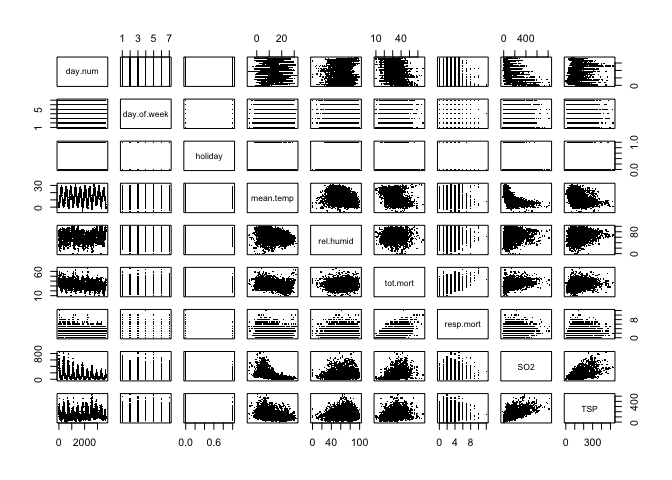
\includegraphics{tema8_files/figure-latex/unnamed-chunk-25-1.pdf}

\begin{Shaded}
\begin{Highlighting}[]
\KeywordTok{faces2}\NormalTok{(USairpollution)}
\end{Highlighting}
\end{Shaded}

\includegraphics{tema8_files/figure-latex/unnamed-chunk-25-2.pdf}

\begin{Shaded}
\begin{Highlighting}[]
\NormalTok{panel.hist <-}\StringTok{ }\NormalTok{function(x, ...) }
\NormalTok{\{ }
          \NormalTok{usr <-}\StringTok{ }\KeywordTok{par}\NormalTok{(}\StringTok{"usr"}\NormalTok{); }\KeywordTok{on.exit}\NormalTok{(}\KeywordTok{par}\NormalTok{(usr)) }
          \KeywordTok{par}\NormalTok{(}\DataTypeTok{usr =} \KeywordTok{c}\NormalTok{(usr[}\DecValTok{1}\NormalTok{:}\DecValTok{2}\NormalTok{], }\DecValTok{0}\NormalTok{, }\FloatTok{1.5}\NormalTok{) ) }
          \NormalTok{h <-}\StringTok{ }\KeywordTok{hist}\NormalTok{(x, }\DataTypeTok{plot =} \OtherTok{FALSE}\NormalTok{) }
          \NormalTok{breaks <-}\StringTok{ }\NormalTok{h$breaks; nB <-}\StringTok{ }\KeywordTok{length}\NormalTok{(breaks) }
          \NormalTok{y <-}\StringTok{ }\NormalTok{h$counts; y <-}\StringTok{ }\NormalTok{y/}\KeywordTok{max}\NormalTok{(y) }
          \KeywordTok{rect}\NormalTok{(breaks[-nB], }\DecValTok{0}\NormalTok{, breaks[-}\DecValTok{1}\NormalTok{], y, }\DataTypeTok{col=}\StringTok{"blue"}\NormalTok{, ...) }
\NormalTok{\} }
\KeywordTok{pairs}\NormalTok{(USairpollution,}\DataTypeTok{diag.panel=}\NormalTok{panel.hist)}
\end{Highlighting}
\end{Shaded}

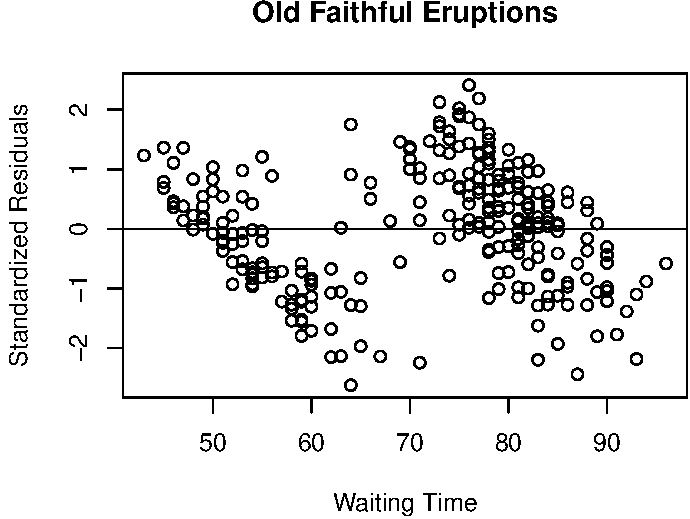
\includegraphics{tema8_files/figure-latex/unnamed-chunk-26-1.pdf}

\begin{Shaded}
\begin{Highlighting}[]
\CommentTok{# Calculo la matriz de correlaciones }
\KeywordTok{cor}\NormalTok{(USairpollution[,-}\DecValTok{1}\NormalTok{]) }
\end{Highlighting}
\end{Shaded}

\begin{verbatim}
##                temp        manu       popul        wind      precip
## temp     1.00000000 -0.19004216 -0.06267813 -0.34973963  0.38625342
## manu    -0.19004216  1.00000000  0.95526935  0.23794683 -0.03241688
## popul   -0.06267813  0.95526935  1.00000000  0.21264375 -0.02611873
## wind    -0.34973963  0.23794683  0.21264375  1.00000000 -0.01299438
## precip   0.38625342 -0.03241688 -0.02611873 -0.01299438  1.00000000
## predays -0.43024212  0.13182930  0.04208319  0.16410559  0.49609671
##             predays
## temp    -0.43024212
## manu     0.13182930
## popul    0.04208319
## wind     0.16410559
## precip   0.49609671
## predays  1.00000000
\end{verbatim}

Otra funcion para calcular PCA en \texttt{princomp}

\begin{Shaded}
\begin{Highlighting}[]
\CommentTok{# Calculo los componentes principales basados en la matriz de correlaciones }
\NormalTok{USair.pc<-}\KeywordTok{princomp}\NormalTok{(USairpollution[,-}\DecValTok{1}\NormalTok{],}\DataTypeTok{cor=}\OtherTok{TRUE}\NormalTok{) }
\KeywordTok{summary}\NormalTok{(USair.pc,}\DataTypeTok{loadings=}\OtherTok{TRUE}\NormalTok{)}
\end{Highlighting}
\end{Shaded}

\begin{verbatim}
## Importance of components:
##                           Comp.1    Comp.2    Comp.3    Comp.4     Comp.5
## Standard deviation     1.4819456 1.2247218 1.1809526 0.8719099 0.33848287
## Proportion of Variance 0.3660271 0.2499906 0.2324415 0.1267045 0.01909511
## Cumulative Proportion  0.3660271 0.6160177 0.8484592 0.9751637 0.99425879
##                             Comp.6
## Standard deviation     0.185599752
## Proportion of Variance 0.005741211
## Cumulative Proportion  1.000000000
## 
## Loadings:
##         Comp.1 Comp.2 Comp.3 Comp.4 Comp.5 Comp.6
## temp     0.330 -0.128  0.672 -0.306  0.558 -0.136
## manu    -0.612 -0.168  0.273  0.137 -0.102 -0.703
## popul   -0.578 -0.222  0.350                0.695
## wind    -0.354  0.131 -0.297 -0.869  0.113       
## precip          0.623  0.505 -0.171 -0.568       
## predays -0.238  0.708         0.311  0.580
\end{verbatim}

\begin{Shaded}
\begin{Highlighting}[]
\CommentTok{#scores}
\KeywordTok{head}\NormalTok{(USair.pc$scores[,}\DecValTok{1}\NormalTok{:}\DecValTok{3}\NormalTok{])}
\end{Highlighting}
\end{Shaded}

\begin{verbatim}
##                 Comp.1      Comp.2     Comp.3
## Albany       0.5389456  0.79206938 -1.3626052
## Albuquerque  1.4170931 -2.86589024 -1.2754003
## Atlanta      0.5989948  0.58723563  0.9954113
## Baltimore   -0.5093800  0.02875397  0.3635995
## Buffalo     -1.3907089  1.88030104 -1.7761919
## Charleston   1.4297533  1.21058365  0.0794435
\end{verbatim}

\begin{Shaded}
\begin{Highlighting}[]
\CommentTok{# PC1 vs PC2}
\KeywordTok{par}\NormalTok{(}\DataTypeTok{pty=}\StringTok{"s"}\NormalTok{) }
\KeywordTok{plot}\NormalTok{(USair.pc$scores[,}\DecValTok{1}\NormalTok{],USair.pc$scores[,}\DecValTok{2}\NormalTok{], }
\DataTypeTok{ylim=}\KeywordTok{range}\NormalTok{(USair.pc$scores[,}\DecValTok{1}\NormalTok{]), }
\DataTypeTok{xlab=}\StringTok{"PC1"}\NormalTok{,}\DataTypeTok{ylab=}\StringTok{"PC2"}\NormalTok{,}\DataTypeTok{type=}\StringTok{"n"}\NormalTok{,}\DataTypeTok{lwd=}\DecValTok{2}\NormalTok{) }
\KeywordTok{text}\NormalTok{(USair.pc$scores[,}\DecValTok{1}\NormalTok{],USair.pc$scores[,}\DecValTok{2}\NormalTok{], }
\DataTypeTok{labels=}\KeywordTok{abbreviate}\NormalTok{(}\KeywordTok{row.names}\NormalTok{(USairpollution)),}\DataTypeTok{cex=}\FloatTok{0.7}\NormalTok{,}\DataTypeTok{lwd=}\DecValTok{2}\NormalTok{)}
\end{Highlighting}
\end{Shaded}

\includegraphics{tema8_files/figure-latex/unnamed-chunk-30-1.pdf}

\begin{Shaded}
\begin{Highlighting}[]
\CommentTok{# PC1 vs PC3}
\KeywordTok{par}\NormalTok{(}\DataTypeTok{pty=}\StringTok{"s"}\NormalTok{) }
\KeywordTok{plot}\NormalTok{(USair.pc$scores[,}\DecValTok{1}\NormalTok{],USair.pc$scores[,}\DecValTok{3}\NormalTok{], }
\DataTypeTok{ylim=}\KeywordTok{range}\NormalTok{(USair.pc$scores[,}\DecValTok{1}\NormalTok{]), }
\DataTypeTok{xlab=}\StringTok{"PC1"}\NormalTok{,}\DataTypeTok{ylab=}\StringTok{"PC3"}\NormalTok{,}\DataTypeTok{type=}\StringTok{"n"}\NormalTok{,}\DataTypeTok{lwd=}\DecValTok{2}\NormalTok{) }
\KeywordTok{text}\NormalTok{(USair.pc$scores[,}\DecValTok{1}\NormalTok{],USair.pc$scores[,}\DecValTok{3}\NormalTok{], }
\DataTypeTok{labels=}\KeywordTok{abbreviate}\NormalTok{(}\KeywordTok{row.names}\NormalTok{(USairpollution)),}\DataTypeTok{cex=}\FloatTok{0.7}\NormalTok{,}\DataTypeTok{lwd=}\DecValTok{2}\NormalTok{)}
\end{Highlighting}
\end{Shaded}

\includegraphics{tema8_files/figure-latex/unnamed-chunk-30-2.pdf}

\begin{Shaded}
\begin{Highlighting}[]
\CommentTok{# PC2 vs PC3}
\KeywordTok{par}\NormalTok{(}\DataTypeTok{pty=}\StringTok{"s"}\NormalTok{) }
\KeywordTok{plot}\NormalTok{(USair.pc$scores[,}\DecValTok{2}\NormalTok{],USair.pc$scores[,}\DecValTok{3}\NormalTok{], }
\DataTypeTok{ylim=}\KeywordTok{range}\NormalTok{(USair.pc$scores[,}\DecValTok{2}\NormalTok{]), }
\DataTypeTok{xlab=}\StringTok{"PC1"}\NormalTok{,}\DataTypeTok{ylab=}\StringTok{"PC3"}\NormalTok{,}\DataTypeTok{type=}\StringTok{"n"}\NormalTok{,}\DataTypeTok{lwd=}\DecValTok{2}\NormalTok{) }
\KeywordTok{text}\NormalTok{(USair.pc$scores[,}\DecValTok{2}\NormalTok{],USair.pc$scores[,}\DecValTok{3}\NormalTok{], }
\DataTypeTok{labels=}\KeywordTok{abbreviate}\NormalTok{(}\KeywordTok{row.names}\NormalTok{(USairpollution)),}\DataTypeTok{cex=}\FloatTok{0.7}\NormalTok{,}\DataTypeTok{lwd=}\DecValTok{2}\NormalTok{)}
\end{Highlighting}
\end{Shaded}

\includegraphics{tema8_files/figure-latex/unnamed-chunk-30-3.pdf}

\subsection{Análisis Cluster}\label{analisis-cluster}

El análisis de cluster es una técnica cuya idea básica es agrupar un
conjunto de observaciones en un número dado de clusters o grupos. Este
agrupamiento se basa en la idea de distancia o similitud entre las
observaciones. Por tanto, la obtención de dichos clusters depende del
criterio o distancia considerados.

Ejemplos de distancias:

\begin{itemize}
\tightlist
\item
  \textbf{Distancia euclídea:} Dados dos objetos \(I_1\) e \(I_2\)
  medidos según dos variables \(x_1\) y \(x_2\), la distancia euclídea
  entre ambos es \[
      d_{I_1,I_2} = \sqrt{(x_{11} - x_{21})^2+(x_{12} - x_{22})^2}  
    \] Con \(p\) dimensiones \[
      d_{I_1,I_2} = \sqrt{\sum_{i=1}^{p}(x_{1k} - x_{2k})^2}  
    \]
\item
  \textbf{Distancia de Mahalanobis:}
\end{itemize}

\[
        d_{I_1,I_2} = (x_i - x_j)^{\prime} W^{-1} (x_i - x_j)
  \] donde \(W\) es la matriz de covarianzas entre las variables. De
este modo, las variables se ponderan según el grado de relación que
exista entre ellas, es decir, si están más o menos correlacionadas. Si
la correlación es nula y las variables están estandarizadas, se obtiene
la distancia euclídea.

\begin{itemize}
\tightlist
\item
  \textbf{Distancia de Minkowski:} \[
    d_{I_1,I_2}^2 = \left[ \sum_{k} |x_{ik} - x_{ij} |^m \right]^{1/m}
    \] donde \(m\) en un número natural, si \(m=1\) la distancia es en
  valor absoluto y \(m=2\) la euclídea.
\end{itemize}

\subsubsection{Métodos de cluster
jerárquicos}\label{metodos-de-cluster-jerarquicos}

En la práctica, no se pueden examinar todas las posibilidades de agrupar
los elementos, incluso con los ordenadores más rápidos. Una solución se
encuentra en los llamados métodos jerárquicos.

\begin{itemize}
\item
  \emph{Métodos aglomerativos:} se comienza con los objetos o individuos
  de modo individual; de este modo, se tienen tantos clusters iniciales
  como objetos. Luego se van agrupando de modo que los primeros en
  hacerlo son los más similares y al final, todos los subgrupos se unen
  en un único cluster.
\item
  \emph{Métodos divisivos o de particionado:} al contrario. Se parte de
  un grupo único con todas las observaciones y se van dividiendo según
  lo lejanos que estén.
\end{itemize}

En cualquier caso, de ambos métodos se deriva un \textbf{dendograma},
que es un gráfico que ilustra cómo se van haciendo las subdivisiones o
los agrupamientos, etapa a etapa.

Consideramos aquí los métodos aglomerativos con diferentes métodos de
unión (linkage methods). Los más importantes son:

\begin{enumerate}
\def\labelenumi{\arabic{enumi}.}
\item
  Mínima distancia o vecino más próximo.
\item
  Máxima distancia o vecino más lejano.
\item
  Distancia media (average distance).
\end{enumerate}

Se puede observar que, de este modo, se define una posible distancia
entre dos clusters: la correspondiente a la pareja de elementos más
cercana, la más lejana o la media de todas las posibles parejas de
elementos de ambos clusters.

\subsubsection{Métodos no jerárquicos}\label{metodos-no-jerarquicos}

Se usan para agrupar objetos, pero no variables, en un conjunto de \(k\)
clusters ya predeterminado. No se tiene que especificar una matriz de
distancias, lo cual entre otras razones permite trabajar con un número
de datos mayor que en el caso de los métodos jerárquicos.

Se parte de un conjunto inicial de clusters elegidos al azar, que son
los representantes de todos ellos; luego se van cambiando de modo
iterativo. Se usa habitualmente el método de las \(k\)-medias.

\textbf{Método de las k-medias} permite asignar a cada observación el
cluster que se encuentra más próximo en términos del centroide (media).
En general, la distancia empleada es la euclídea.

Pasos:

\begin{enumerate}
\def\labelenumi{\arabic{enumi}.}
\item
  Se toman al azar \(k\) clusters iniciales.
\item
  Para el conjunto de observaciones, se vuelve a calcular las distancias
  a los centroides de los clusters y se reasignan a los que estén más
  próximos. Se vuelven a recalcular los centroides de los \(k\) clusters
  después de las reasignaciones de los elementos.
\item
  Se repiten los dos pasos anteriores hasta que no se produzca ninguna
  reasignación, es decir, hasta que los elementos se estabilicen en
  algún grupo. Usualmente, se especifican \(k\) centroides iniciales y
  se procede al paso (2) y, en la práctica, se observan la mayor parte
  de reasignaciones en las primeras iteraciones.
\end{enumerate}

\#\#\# Ejemplos:

En este conjunto de datos se observa la composición de diferentes vinos.

\begin{Shaded}
\begin{Highlighting}[]
\CommentTok{# install.packages('rattle')}
\KeywordTok{data}\NormalTok{(wine, }\DataTypeTok{package=}\StringTok{'rattle'}\NormalTok{)}
\KeywordTok{head}\NormalTok{(wine)}
\end{Highlighting}
\end{Shaded}

\begin{verbatim}
##   Type Alcohol Malic  Ash Alcalinity Magnesium Phenols Flavanoids
## 1    1   14.23  1.71 2.43       15.6       127    2.80       3.06
## 2    1   13.20  1.78 2.14       11.2       100    2.65       2.76
## 3    1   13.16  2.36 2.67       18.6       101    2.80       3.24
## 4    1   14.37  1.95 2.50       16.8       113    3.85       3.49
## 5    1   13.24  2.59 2.87       21.0       118    2.80       2.69
## 6    1   14.20  1.76 2.45       15.2       112    3.27       3.39
##   Nonflavanoids Proanthocyanins Color  Hue Dilution Proline
## 1          0.28            2.29  5.64 1.04     3.92    1065
## 2          0.26            1.28  4.38 1.05     3.40    1050
## 3          0.30            2.81  5.68 1.03     3.17    1185
## 4          0.24            2.18  7.80 0.86     3.45    1480
## 5          0.39            1.82  4.32 1.04     2.93     735
## 6          0.34            1.97  6.75 1.05     2.85    1450
\end{verbatim}

Siempre es recomendable estandarizar las variables

\begin{Shaded}
\begin{Highlighting}[]
\NormalTok{wine.stand <-}\StringTok{ }\KeywordTok{scale}\NormalTok{(wine[-}\DecValTok{1}\NormalTok{])  }\CommentTok{# To standarize the variables}

\CommentTok{# K-Means}
\NormalTok{k.means.fit <-}\StringTok{ }\KeywordTok{kmeans}\NormalTok{(wine.stand, }\DecValTok{3}\NormalTok{) }\CommentTok{# k = 3}
\end{Highlighting}
\end{Shaded}

\begin{Shaded}
\begin{Highlighting}[]
\KeywordTok{attributes}\NormalTok{(k.means.fit)}
\end{Highlighting}
\end{Shaded}

\begin{verbatim}
## $names
## [1] "cluster"      "centers"      "totss"        "withinss"    
## [5] "tot.withinss" "betweenss"    "size"         "iter"        
## [9] "ifault"      
## 
## $class
## [1] "kmeans"
\end{verbatim}

\begin{verbatim}
##      Alcohol      Malic        Ash Alcalinity   Magnesium     Phenols
## 1  0.8328826 -0.3029551  0.3636801 -0.6084749  0.57596208  0.88274724
## 2  0.1644436  0.8690954  0.1863726  0.5228924 -0.07526047 -0.97657548
## 3 -0.9234669 -0.3929331 -0.4931257  0.1701220 -0.49032869 -0.07576891
##    Flavanoids Nonflavanoids Proanthocyanins      Color        Hue
## 1  0.97506900   -0.56050853      0.57865427  0.1705823  0.4726504
## 2 -1.21182921    0.72402116     -0.77751312  0.9388902 -1.1615122
## 3  0.02075402   -0.03343924      0.05810161 -0.8993770  0.4605046
##     Dilution    Proline
## 1  0.7770551  1.1220202
## 2 -1.2887761 -0.4059428
## 3  0.2700025 -0.7517257
\end{verbatim}

\begin{verbatim}
##   [1] 1 1 1 1 1 1 1 1 1 1 1 1 1 1 1 1 1 1 1 1 1 1 1 1 1 1 1 1 1 1 1 1 1 1 1
##  [36] 1 1 1 1 1 1 1 1 1 1 1 1 1 1 1 1 1 1 1 1 1 1 1 1 3 3 2 3 3 3 3 3 3 3 3
##  [71] 3 3 3 1 3 3 3 3 3 3 3 3 3 2 3 3 3 3 3 3 3 3 3 3 3 1 3 3 3 3 3 3 3 3 3
## [106] 3 3 3 3 3 3 3 3 3 3 3 3 3 2 3 3 1 3 3 3 3 3 3 3 3 2 2 2 2 2 2 2 2 2 2
## [141] 2 2 2 2 2 2 2 2 2 2 2 2 2 2 2 2 2 2 2 2 2 2 2 2 2 2 2 2 2 2 2 2 2 2 2
## [176] 2 2 2
\end{verbatim}

\begin{verbatim}
## [1] 62 51 65
\end{verbatim}

Una pregunta fundamental es cómo determinar el valor del parámetro
\(k\). Si consideramos el porcentaje de varianza explicado como una
función del número de grupos:

Uno debe elegir un número de grupos de modo que la adición de otro grupo
no da mucho mejor modelado de los datos. Más precisamente, si se traza
el porcentaje de varianza explicado por los conglomerados en función del
número de racimos, los primeros grupos agregarán mucha información
(explican mucha varianza), pero en algún momento la ganancia marginal
disminuirá, dando un ángulo en la gráfico. El número de racimos se elige
en este punto, de ahí el ``criterio del codo''.

\begin{Shaded}
\begin{Highlighting}[]
\NormalTok{wssplot <-}\StringTok{ }\NormalTok{function(data, }\DataTypeTok{nc=}\DecValTok{15}\NormalTok{, }\DataTypeTok{seed=}\DecValTok{1234}\NormalTok{)\{}
  \NormalTok{wss <-}\StringTok{ }\NormalTok{(}\KeywordTok{nrow}\NormalTok{(data)-}\DecValTok{1}\NormalTok{)*}\KeywordTok{sum}\NormalTok{(}\KeywordTok{apply}\NormalTok{(data,}\DecValTok{2}\NormalTok{,var))}
  \NormalTok{for (i in }\DecValTok{2}\NormalTok{:nc)\{}
    \KeywordTok{set.seed}\NormalTok{(seed)}
    \NormalTok{wss[i] <-}\StringTok{ }\KeywordTok{sum}\NormalTok{(}\KeywordTok{kmeans}\NormalTok{(data, }\DataTypeTok{centers=}\NormalTok{i)$withinss)\}}
  \KeywordTok{plot}\NormalTok{(}\DecValTok{1}\NormalTok{:nc, wss, }\DataTypeTok{type=}\StringTok{"b"}\NormalTok{, }\DataTypeTok{xlab=}\StringTok{"Number of Clusters"}\NormalTok{,}
       \DataTypeTok{ylab=}\StringTok{"Within groups sum of squares"}\NormalTok{)\}}

\KeywordTok{wssplot}\NormalTok{(wine.stand, }\DataTypeTok{nc=}\DecValTok{6}\NormalTok{) }
\end{Highlighting}
\end{Shaded}

\includegraphics{tema8_files/figure-latex/unnamed-chunk-35-1.pdf}

La \texttt{library(cluster)} permite (con el paso previo de un PCA)
representar los clusters en 2 dimensiones

\begin{Shaded}
\begin{Highlighting}[]
\KeywordTok{library}\NormalTok{(cluster)}
\KeywordTok{clusplot}\NormalTok{(wine.stand, k.means.fit$cluster, }
         \DataTypeTok{main=}\StringTok{'2D representation of the Cluster solution'}\NormalTok{,}
         \DataTypeTok{color=}\OtherTok{TRUE}\NormalTok{, }\DataTypeTok{shade=}\OtherTok{TRUE}\NormalTok{,}
         \DataTypeTok{labels=}\DecValTok{2}\NormalTok{, }\DataTypeTok{lines=}\DecValTok{0}\NormalTok{)}
\end{Highlighting}
\end{Shaded}

\includegraphics{tema8_files/figure-latex/unnamed-chunk-36-1.pdf}

Sabiendo que hay tres tipos de vinos \texttt{wine\$Type}, podemos
calcular una matriz de confusión

\begin{Shaded}
\begin{Highlighting}[]
\KeywordTok{table}\NormalTok{(wine$Type)}
\end{Highlighting}
\end{Shaded}

\begin{verbatim}
## 
##  1  2  3 
## 59 71 48
\end{verbatim}

\begin{Shaded}
\begin{Highlighting}[]
\KeywordTok{table}\NormalTok{(wine[,}\DecValTok{1}\NormalTok{],k.means.fit$cluster)}
\end{Highlighting}
\end{Shaded}

\begin{verbatim}
##    
##      1  2  3
##   1 59  0  0
##   2  3  3 65
##   3  0 48  0
\end{verbatim}

\textbf{Cluster jerarquico}

Los métodos jerárquicos utilizan una matriz de distancia como una input
para el algoritmo de agrupación. La elección de una métrica apropiada
influirá en la forma de los clusters, ya que algunos elementos pueden
estar cerca uno del otro según una distancia y más lejos de acuerdo con
otro.

\begin{Shaded}
\begin{Highlighting}[]
\NormalTok{d <-}\StringTok{ }\KeywordTok{dist}\NormalTok{(wine.stand, }\DataTypeTok{method =} \StringTok{"euclidean"}\NormalTok{) }\CommentTok{# Euclidean distance matrix.}
\end{Highlighting}
\end{Shaded}

Ward's minimum variance criterion minimizes the total within-cluster
variance

\begin{Shaded}
\begin{Highlighting}[]
\NormalTok{H.fit <-}\StringTok{ }\KeywordTok{hclust}\NormalTok{(d, }\DataTypeTok{method=}\StringTok{"ward"}\NormalTok{)}
\end{Highlighting}
\end{Shaded}

\begin{verbatim}
## The "ward" method has been renamed to "ward.D"; note new "ward.D2"
\end{verbatim}

\begin{Shaded}
\begin{Highlighting}[]
\KeywordTok{class}\NormalTok{(H.fit)}
\end{Highlighting}
\end{Shaded}

\begin{verbatim}
## [1] "hclust"
\end{verbatim}

La opcion \texttt{plot} de un objeto \texttt{hclust} nos devuelve el
dendograma:

\begin{Shaded}
\begin{Highlighting}[]
\KeywordTok{plot}\NormalTok{(H.fit) }\CommentTok{# display dendogram}
\NormalTok{groups <-}\StringTok{ }\KeywordTok{cutree}\NormalTok{(H.fit, }\DataTypeTok{k=}\DecValTok{3}\NormalTok{) }\CommentTok{# cut tree into 5 clusters}
\CommentTok{# draw dendogram with red borders around the 5 clusters}
\KeywordTok{rect.hclust}\NormalTok{(H.fit, }\DataTypeTok{k=}\DecValTok{3}\NormalTok{, }\DataTypeTok{border=}\StringTok{"red"}\NormalTok{) }
\end{Highlighting}
\end{Shaded}

\includegraphics{tema8_files/figure-latex/unnamed-chunk-40-1.pdf}

\begin{Shaded}
\begin{Highlighting}[]
\KeywordTok{table}\NormalTok{(wine[,}\DecValTok{1}\NormalTok{],groups)}
\end{Highlighting}
\end{Shaded}

\begin{verbatim}
##    groups
##      1  2  3
##   1 58  1  0
##   2  7 58  6
##   3  0  0 48
\end{verbatim}

\subsection{Análisis de Series
temporales}\label{analisis-de-series-temporales}

\texttt{R} tiene amplias facilidades para analizar datos de series
temporales. Esta sección describe la creación de una serie de tiempo,
descomposición estacional, predicción con el paquete \texttt{forecast}.

\begin{Shaded}
\begin{Highlighting}[]
\CommentTok{# save a numeric vector containing 84 monthly observations}
\CommentTok{# from Jan 2009 to Dec 2015 as a time series object}
\KeywordTok{set.seed}\NormalTok{(}\DecValTok{1234}\NormalTok{)}
\NormalTok{myvector <-}\StringTok{ }\KeywordTok{rnorm}\NormalTok{(}\DecValTok{84}\NormalTok{) }
\NormalTok{myts <-}\StringTok{ }\KeywordTok{ts}\NormalTok{(myvector, }\DataTypeTok{start=}\KeywordTok{c}\NormalTok{(}\DecValTok{2009}\NormalTok{, }\DecValTok{1}\NormalTok{), }\DataTypeTok{end=}\KeywordTok{c}\NormalTok{(}\DecValTok{2015}\NormalTok{, }\DecValTok{12}\NormalTok{), }\DataTypeTok{frequency=}\DecValTok{12}\NormalTok{)}
\KeywordTok{class}\NormalTok{(myts)}
\end{Highlighting}
\end{Shaded}

\begin{verbatim}
## [1] "ts"
\end{verbatim}

\begin{Shaded}
\begin{Highlighting}[]
\CommentTok{# subset the time series (June 2014 to December 2014)}
\NormalTok{myts2 <-}\StringTok{ }\KeywordTok{window}\NormalTok{(myts, }\DataTypeTok{start=}\KeywordTok{c}\NormalTok{(}\DecValTok{2014}\NormalTok{, }\DecValTok{6}\NormalTok{), }\DataTypeTok{end=}\KeywordTok{c}\NormalTok{(}\DecValTok{2014}\NormalTok{, }\DecValTok{12}\NormalTok{))}
\CommentTok{# plot series}
\KeywordTok{plot}\NormalTok{(myts)}
\end{Highlighting}
\end{Shaded}

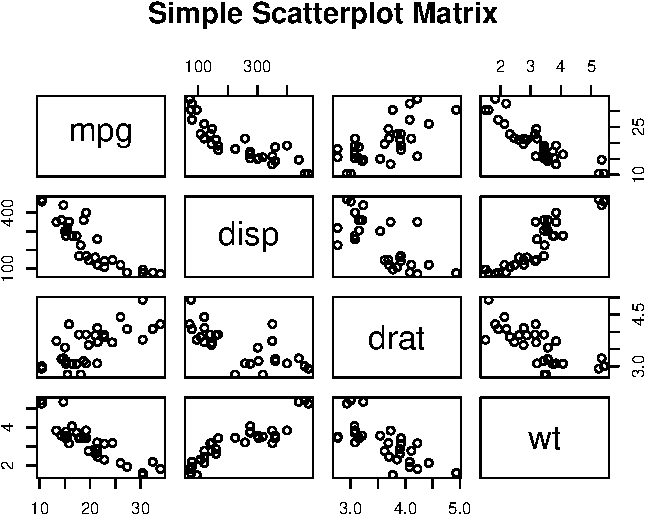
\includegraphics{tema8_files/figure-latex/unnamed-chunk-42-1.pdf}

Ejemplo con datos reales:

\begin{Shaded}
\begin{Highlighting}[]
\KeywordTok{data}\NormalTok{(AirPassengers)}
\KeywordTok{class}\NormalTok{(AirPassengers)}
\end{Highlighting}
\end{Shaded}

\begin{verbatim}
## [1] "ts"
\end{verbatim}

\begin{Shaded}
\begin{Highlighting}[]
\NormalTok{?AirPassengers}
\KeywordTok{start}\NormalTok{(AirPassengers)}
\end{Highlighting}
\end{Shaded}

\begin{verbatim}
## [1] 1949    1
\end{verbatim}

\begin{Shaded}
\begin{Highlighting}[]
\KeywordTok{end}\NormalTok{(AirPassengers)}
\end{Highlighting}
\end{Shaded}

\begin{verbatim}
## [1] 1960   12
\end{verbatim}

\begin{Shaded}
\begin{Highlighting}[]
\KeywordTok{frequency}\NormalTok{(AirPassengers)}
\end{Highlighting}
\end{Shaded}

\begin{verbatim}
## [1] 12
\end{verbatim}

\begin{Shaded}
\begin{Highlighting}[]
\KeywordTok{cycle}\NormalTok{(AirPassengers)}
\end{Highlighting}
\end{Shaded}

\begin{verbatim}
##      Jan Feb Mar Apr May Jun Jul Aug Sep Oct Nov Dec
## 1949   1   2   3   4   5   6   7   8   9  10  11  12
## 1950   1   2   3   4   5   6   7   8   9  10  11  12
## 1951   1   2   3   4   5   6   7   8   9  10  11  12
## 1952   1   2   3   4   5   6   7   8   9  10  11  12
## 1953   1   2   3   4   5   6   7   8   9  10  11  12
## 1954   1   2   3   4   5   6   7   8   9  10  11  12
## 1955   1   2   3   4   5   6   7   8   9  10  11  12
## 1956   1   2   3   4   5   6   7   8   9  10  11  12
## 1957   1   2   3   4   5   6   7   8   9  10  11  12
## 1958   1   2   3   4   5   6   7   8   9  10  11  12
## 1959   1   2   3   4   5   6   7   8   9  10  11  12
## 1960   1   2   3   4   5   6   7   8   9  10  11  12
\end{verbatim}

\begin{Shaded}
\begin{Highlighting}[]
\KeywordTok{plot}\NormalTok{(AirPassengers)}
\end{Highlighting}
\end{Shaded}

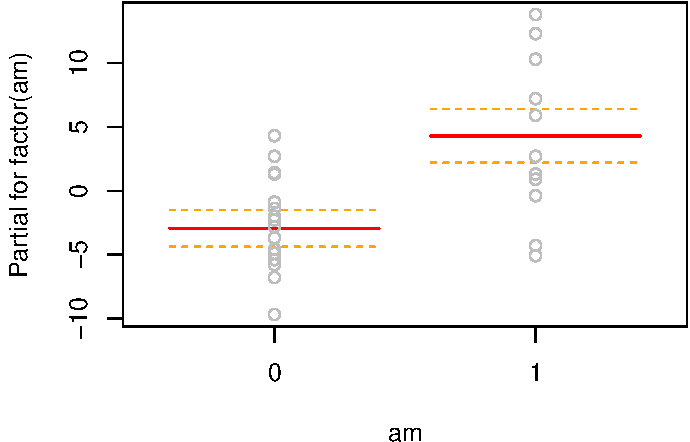
\includegraphics{tema8_files/figure-latex/unnamed-chunk-43-1.pdf}

\textbf{¿Qué patrones ves?}

La tendencia interanual muestra claramente que el número de pasajeros ha
ido en aumento.

\begin{Shaded}
\begin{Highlighting}[]
\CommentTok{# plot of aggregated by months}
\KeywordTok{plot}\NormalTok{(}\KeywordTok{aggregate}\NormalTok{(AirPassengers,}\DataTypeTok{FUN=}\NormalTok{mean))}
\end{Highlighting}
\end{Shaded}

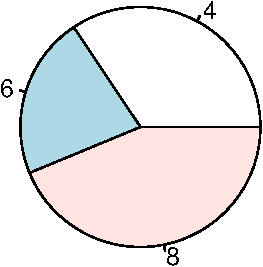
\includegraphics{tema8_files/figure-latex/unnamed-chunk-44-1.pdf} La
varianza y el valor medio en julio y agosto es mucho mayor que el resto
de los meses.

\begin{Shaded}
\begin{Highlighting}[]
\CommentTok{# boxplots accross months will show seasonal effects}
\KeywordTok{boxplot}\NormalTok{(AirPassengers~}\KeywordTok{cycle}\NormalTok{(AirPassengers))}
\end{Highlighting}
\end{Shaded}

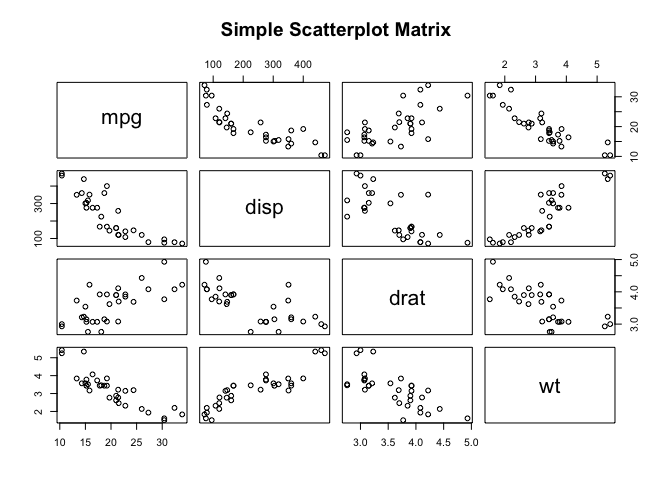
\includegraphics{tema8_files/figure-latex/unnamed-chunk-45-1.pdf}
También observamos un fuerte efecto estacional con un ciclo de 12 meses
o menos.

La función \texttt{decompose()} descompone una serie de tiempo en la
estacionalidad, la tendencia y los componentes irregulares utilizando
promedios móviles. El componente estacional puede ser aditivo: \[
      Y_t = T_t + S_t + e_t
\]

\subsubsection{\texorpdfstring{La libreria
\texttt{forecast}}{La libreria forecast}}\label{la-libreria-forecast}

\begin{Shaded}
\begin{Highlighting}[]
\KeywordTok{library}\NormalTok{(forecast)}
\NormalTok{tsData <-}\StringTok{ }\NormalTok{EuStockMarkets[, }\DecValTok{1}\NormalTok{] }\CommentTok{# ts data}
\NormalTok{decomposedRes <-}\StringTok{ }\KeywordTok{decompose}\NormalTok{(tsData,}
                           \DataTypeTok{type=}\StringTok{"mult"}\NormalTok{)}
                \CommentTok{# use type = "additive" for additive components}
\KeywordTok{plot} \NormalTok{(decomposedRes) }\CommentTok{# see plot below}
\end{Highlighting}
\end{Shaded}

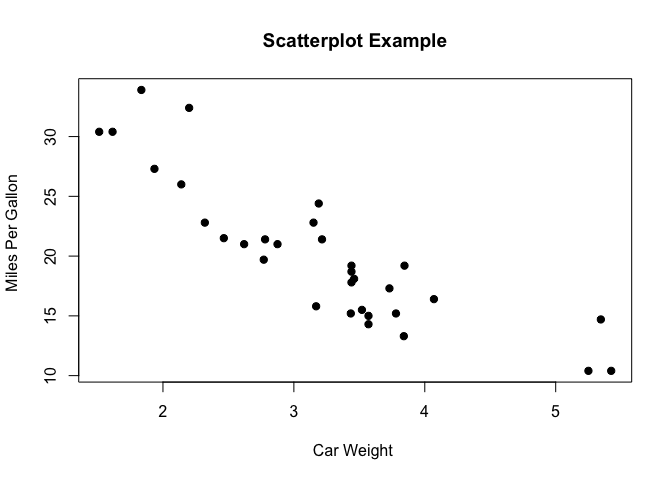
\includegraphics{tema8_files/figure-latex/unnamed-chunk-46-1.pdf}

\begin{Shaded}
\begin{Highlighting}[]
\NormalTok{stlRes <-}\StringTok{ }\KeywordTok{stl}\NormalTok{(tsData, }\DataTypeTok{s.window =} \StringTok{"periodic"}\NormalTok{)}
\end{Highlighting}
\end{Shaded}

\begin{Shaded}
\begin{Highlighting}[]
\KeywordTok{library}\NormalTok{(forecast)}
\NormalTok{ts.stl <-}\StringTok{ }\KeywordTok{stl}\NormalTok{(AirPassengers,}\StringTok{"periodic"}\NormalTok{)  }\CommentTok{# decompose the TS}
\NormalTok{ts.sa <-}\StringTok{ }\KeywordTok{seasadj}\NormalTok{(ts.stl)  }\CommentTok{# de-seasonalize}
\KeywordTok{plot}\NormalTok{(AirPassengers, }\DataTypeTok{type=}\StringTok{"l"}\NormalTok{)  }\CommentTok{# original series}
\end{Highlighting}
\end{Shaded}

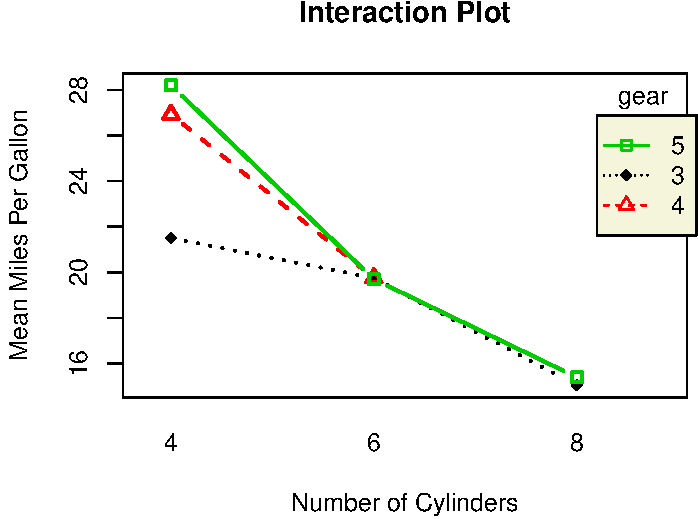
\includegraphics{tema8_files/figure-latex/unnamed-chunk-47-1.pdf}

\begin{Shaded}
\begin{Highlighting}[]
\KeywordTok{plot}\NormalTok{(ts.sa, }\DataTypeTok{type=}\StringTok{"l"}\NormalTok{)  }\CommentTok{# seasonal adjusted}
\end{Highlighting}
\end{Shaded}

\includegraphics{tema8_files/figure-latex/unnamed-chunk-47-2.pdf}

\begin{Shaded}
\begin{Highlighting}[]
\KeywordTok{seasonplot}\NormalTok{(ts.sa, }\DecValTok{12}\NormalTok{, }\DataTypeTok{col=}\KeywordTok{rainbow}\NormalTok{(}\DecValTok{12}\NormalTok{), }\DataTypeTok{year.labels=}\OtherTok{TRUE}\NormalTok{,}
          \DataTypeTok{main=}\StringTok{"Seasonal plot: Airpassengers"}\NormalTok{)}
\end{Highlighting}
\end{Shaded}

\includegraphics{tema8_files/figure-latex/unnamed-chunk-47-3.pdf}

\begin{Shaded}
\begin{Highlighting}[]
              \CommentTok{# seasonal frequency set as 12 for monthly data.}
\end{Highlighting}
\end{Shaded}

\begin{Shaded}
\begin{Highlighting}[]
\KeywordTok{library}\NormalTok{(forecast)}
\KeywordTok{plot}\NormalTok{(}\KeywordTok{forecast}\NormalTok{(ts.stl,}\DataTypeTok{h=}\DecValTok{10}\NormalTok{))}
\end{Highlighting}
\end{Shaded}

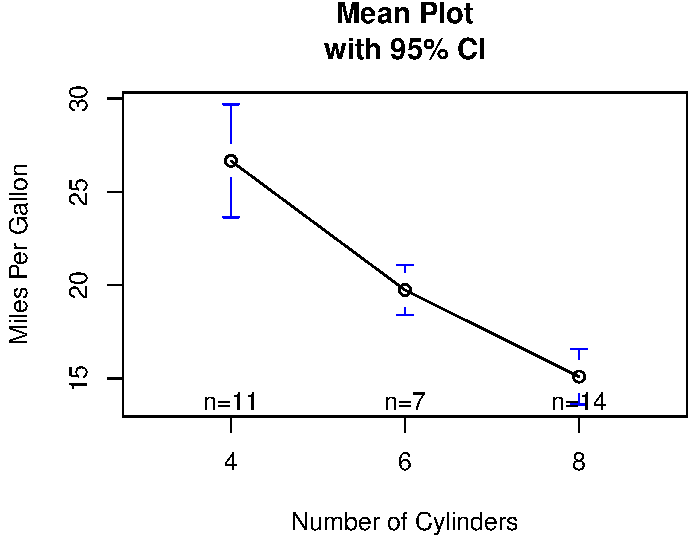
\includegraphics{tema8_files/figure-latex/unnamed-chunk-48-1.pdf}

\end{document}